
\documentclass[12 pt ,a4 paper, openright, oneside]{book}

% Pacchetti %
\usepackage[italian]{babel} % Italiano
\usepackage[utf8]{inputenc}
\usepackage{csquotes}
\usepackage{hyperref}
\usepackage{subcaption}
\usepackage{hyphenat}
\usepackage[hypcap=true]{caption}
\usepackage{setspace}
\usepackage[hang,flushmargin,bottom]{footmisc}
\usepackage{todonotes} % Note Todo
\usepackage{soul} % strikethrough 
\usepackage{caption}
\usepackage{placeins}
\usepackage{amssymb,amsmath}
\usepackage[official]{eurosym}
\usepackage{frontespizio}
\usepackage{booktabs}
\usepackage{listings}
\renewcommand{\lstlistingname}{Codice}% Listing -> Codice
\usepackage{mdframed}
\def\checkmark{\tikz\fill[scale=0.4](0,.35) -- (.25,0) -- (1,.7) -- (.25,.15) -- cycle;}
\usepackage{eurosym}
% Tabelle %
\usepackage[normalem]{ulem}
\useunder{\uline}{\ul}{}
\usepackage{array,ragged2e}
\usepackage{colortbl}
\newcolumntype{P}[1]{>{\RaggedRight\arraybackslash}p{#1}}

% Immagini %
\usepackage{graphicx, wrapfig, float, rotating}
% \graphicspath{{images/}}

% Bibliografia %
\usepackage[backend=biber,style=numeric,sorting=none]{biblatex}
\addbibresource{bibliografia.bib}

\begin{document}

% Qui ci andrà il frontespizio

\begin{titlepage}
\begin{center}
    \begin{figure}
        \centering
        
\includegraphics[width=0.35\textwidth]{Images/logo.jpg}
    \end{figure}
    \begin{LARGE}
        {
        \bf Universit\`a degli Studi di Pisa
        }
        \\
        \vskip 0.1cm
    \end{LARGE}
%    \rule{15cm}{0.03cm}

    \begin{Large}
    \textbf {Dipartimento di Informatica}\\
    \end{Large}

    \begin{Large}
    \vskip 0.3cm
    Corso di Laurea Triennale in Informatica
    \end{Large}

\vskip 2cm
\begin{LARGE}
{\bf Studio del Dust Attack: un attacco all'anonimato di Bitcoin}
\\[3mm]
% {\bf V 0.1 - ultima modifica 14/12/2021}
% \\[3mm]
% {\bf A QUALIT\`A GARANTITA}
% \\[3mm]
%{\bf }
%\\[2mm]
\end{LARGE}

\vskip 2cm

\begin{tabular}{lr}
\normalsize  \textit{Candidato}: &\normalsize \textit{Relatori/Relatrici}:
\\[4mm] \large Jacopo Raffi &\normalsize \hspace{1.5cm}Prof.ssa \large Laura Emilia Maria Ricci

% \\[4mm] \normalsize { }                &\hspace{1cm} \normalsize Correlatori:
\\[3mm] \large                 &\hspace{1.5cm} \normalsize
Prof. \large Damiano Di Francesco Maesa 

\end{tabular}

\vskip 2cm

\begin{large}
%\rule{15cm}{0.03cm}\\[2mm]
Anno Accademico 2021-2022
%\rule{15cm}{0.03cm}\\
\end{large}

\end{center}
\end{titlepage}

% .. fine frontespizio


\tableofcontents

% il capitolo inizia a pagina nuova. Usare il comando \input{} per aggiungere senza andare a pagina nuova
\definecolor{lightgray}{rgb}{.9,.9,.9}
\definecolor{darkgray}{rgb}{.4,.4,.4}
\definecolor{purple}{rgb}{0.65, 0.12, 0.82}

\lstdefinelanguage{Python}{
  keywords={True, False, catch, def, float, or, len, not, return, None, if, in, while, do, for, elif, else, break, lambda},
  keywordstyle=\color{blue}\bfseries,
  ndkeywords={class, export, boolean, throw, implements, import, this},
  ndkeywordstyle=\color{teal}\bfseries,
  identifierstyle=\color{black},
  sensitive=false,
  comment=[l]{#},
  morecomment=[s]{"""}{"""},
  commentstyle=\color{purple}\ttfamily,
  stringstyle=\color{red}\ttfamily,
  morestring=[b]',
  morestring=[b]"
}

\lstset{
   language=Python,
   backgroundcolor=\color{lightgray},
   extendedchars=true,
   basicstyle=\footnotesize\ttfamily,
   showstringspaces=false,
   showspaces=false,
   numbers=left,
   numberstyle=\footnotesize,
   numbersep=9pt,
   tabsize=2,
   breaklines=true,
   showtabs=false,
   captionpos=b
}

\setstretch{1.2}
\chapter*{Ringraziamenti} % L'asterisco permette di non indicizzare il capitolo (e quindi non gli da un numero)
\begin{flushright}
\itshape 
Fill me
\end{flushright}


\chapter{Introduzione}
 
\chapter{Background}
In questo capitolo verrà descritta la tecnologia alla base di Bitcoin. Particolare attenzione verrà data alla blockchain, la struttura dati che costituisce il libro contabile, al funzionamento delle transazioni, agli indirizzi per esporre infine la questione relativa all'anonimato. 
%1- Spiegare cosa sono i btcoin("storia" ecc...)
%2- Spiegare la blockchain(definizione)
%3- Spiegare address, wallet(anonimato), generazione indirizzi
%4- concentrarsi sulle transazioni(differenza teoria e pratica anonimato), come avvengono come funzionano %la fee ecc...
%Ricorda di mettere immagini
\section{Bitcoin}
Bitcoin, l’unità monetaria elettronica a cui facciamo riferimento in questa tesi, è stata sviluppata da Satoshi Nakamoto, un misterioso autore giapponese la cui identità resta a tutt'oggi ignota, tanto da indurre molti a pensare che si tratti di uno pseudonimo, o che dietro a tale nome si celi in realtà non una singola persona, ma addirittura un gruppo di ricercatori o di informatici. L’articolo in cui viene presentato l’intero protocollo Bitcoin viene pubblicato nel 2008, sotto il nome di ”Bitcoin: A Peer-to-Peer Electronic Cash System”\cite{nakamoto2009bitcoin}; il paper è facilmente reperibile e contiene la descrizione dettagliata del protocollo alla base del funzionamento di Bitcoin.\\La peculiarità di tale sistema è l’uso di una rete secondo il modello Peer-to-Peer per effettuare, diffondere e validare le transazioni, e l’intero storico di esse viene mantenuto in un libro contabile distribuito e di pubblica consultazione. La grande e difficile sfida che Bitcoin dunque si pone è quella di coniugare l’anonimato degli utenti con un’alta affidabilità relativamente alle transazioni e alla loro validità e integrità.\\A fronte della sfida di trasparenza versus affidabilità, è fondamentale definire un’implementazione del libro contabile che impedisca alterazioni di transazioni già registrate e validate: ricordiamo che in questo contesto paritario e distribuito, nessun controllo viene effettuato da parte di entità centrali, come per esempio le banche.\\
La soluzione ideata da Nakamoto per garantire l’integrità dello storico delle transazioni è stata quella di implementare il libro contabile tramite una particolare struttura dati: la blockchain.\\Come suggerisce il nome, la struttura si compone di una serie di blocchi collegati tra di loro come in una catena: ogni blocco racchiude un insieme di transazioni effettuate in un certo periodo temporale.\\Il blocco corrente, non ancora inserito, contiene le ultime transazioni la cui legittimazione deve essere ancora approvata, mentre i blocchi precedenti, già
agganciati alla catena, si riferiscono a transazioni già validate, e la blockchain è fin lì immutabile. Il meccanismo che garantisce la totale immutabilità della struttura, pena la sua completa invalidazione, è la crittografia.\\\\
\begin{figure}[h!]
    \centering
    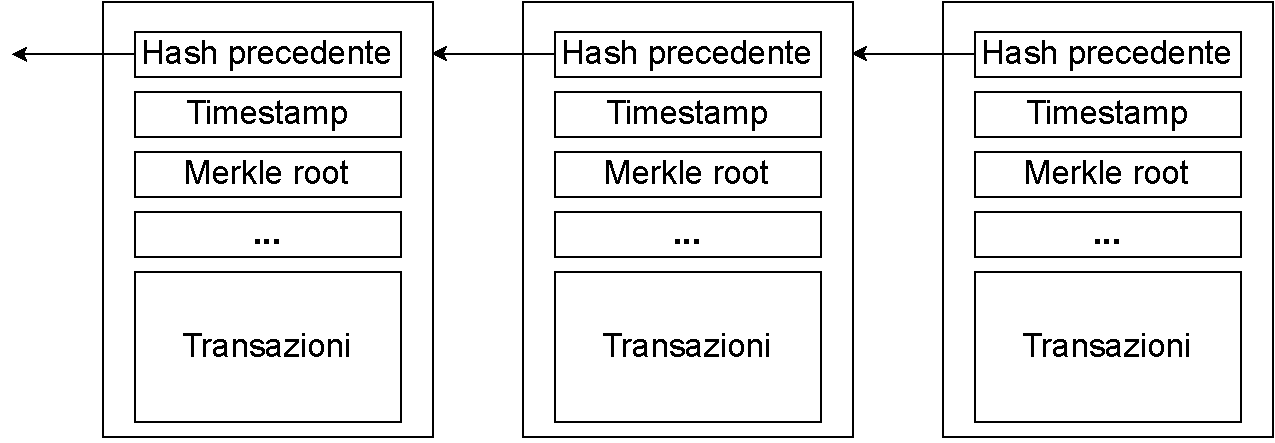
\includegraphics[scale=0.6]{Images/blockChaining.pdf}
    \caption{Schema della Blockchain}
    \label{fig:blockchain}
\end{figure}
\FloatBarrier
\section{Blockchain}
Un generico blocco Bi all’interno della blockchain contiene la sequenza di transazioni relative ad un certo periodo temporale (supponiamo che siano n: T1 , T2 , ... ,Tn ) e un valore hash $h_{i-1}$ identificativo del blocco precedente nella catena, che è l’output di una funzione hash crittografica (la cui definizione sarà data nel seguito).\\È inoltre presente un campo detto nonce, che servirà per l’operazione di mining, ovvero il procedimento che porta all’aggiunta di un nuovo blocco alla blockchain. Sono presenti anche altri dati all’interno del blocco, ma al fine di descrivere il meccanismo crittografico che salvaguarda l’integrità della struttura questo livello di dettaglio è sufficiente.\\\\\\In Figura \ref{fig:blocchi} è rappresentata la struttura di un generico blocco Bi all’interno della blockchain.
\begin{figure}[h!]
    \centering
    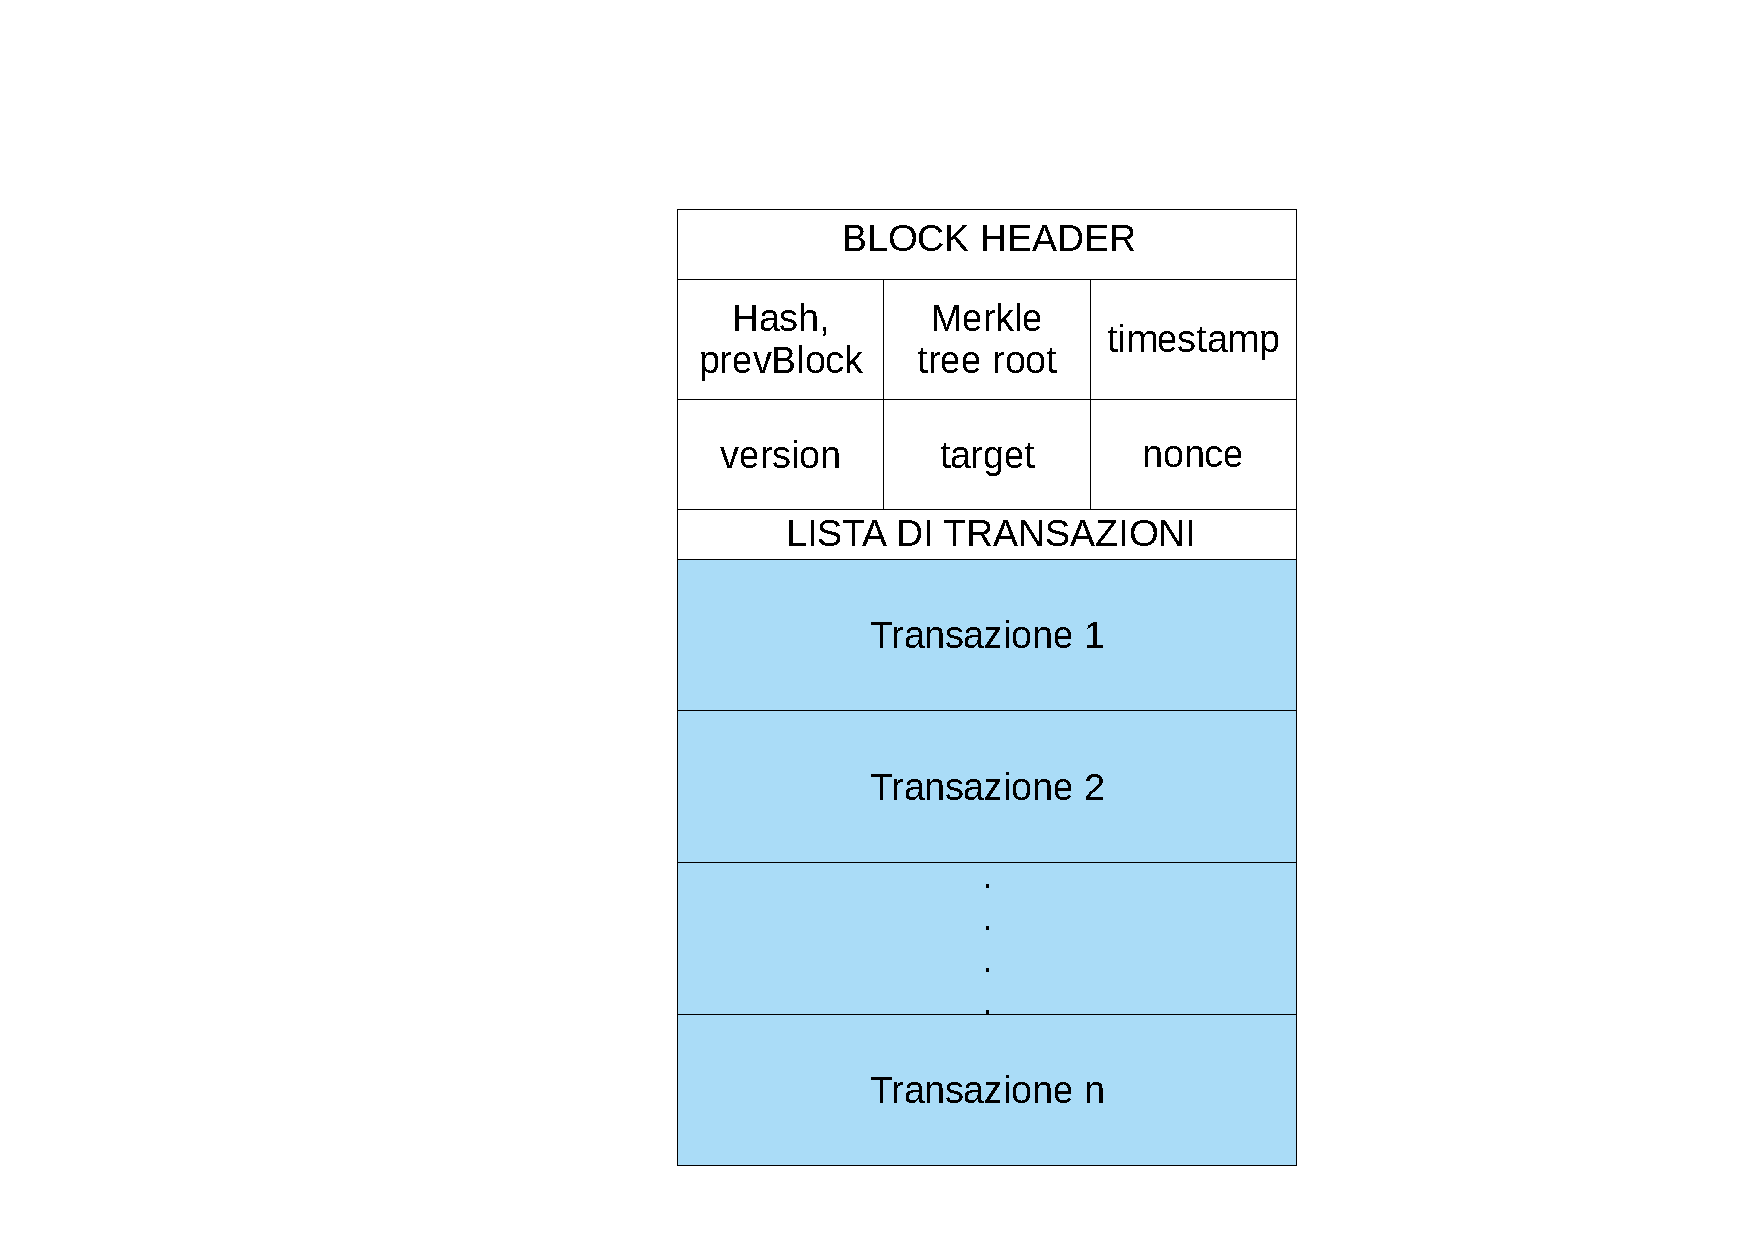
\includegraphics[scale=0.4, trim = 0cm 0cm 0cm 3cm, clip]{Images/blocco_singolo.pdf}
    \caption{Schema di un generico blocco}
    \label{fig:blocchi}
\end{figure}
\FloatBarrier
Come accennato sopra, ogni blocco ha un suo identificativo univoco, una sor-
ta di impronta digitale personale, che è l’output di una opportuna funzione
hash.\\
Una funzione hash $f$: X $\longrightarrow$ Y è una funzione matematica avente come dominio X e codominio Y, insiemi finiti tali che $|X| >> |Y |$.\\Tale funzione prende in input elementi di X di lunghezza qualsiasi e produce in output, a prescindere dalla lunghezza dell’input, stringhe binarie di dimensione fissa, i cosiddetti fingerprint, chiamati anche immagini hash o semplicemente hash.\\
Una proprietà fondamentale delle funzioni hash è relativa al tempo necessario al loro calcolo: devono essere calcolate efficientemente, ossia a fronte di un input di $m$ bit, la complessità computazionale per produrne il fingerprint deve essere $O(m)$, lineare o comunque polinomiale nei bit su cui è rappresentato l’input.\\ Vista la grande differenza di cardinalità tra i due insiemi X e Y, inevitabilmente alcuni input diversi della funzione hash avranno la stessa immagine; questo fenomeno è detto collisione: $x_1$ e $x_2$ $\in$ X, con $x_1 \neq x2$ , collidono se la loro immagine hash è la stessa ( f ($x_1$ ) = f ($x_2$ ) ).\\In crittografia si usano alcune famiglie di funzioni hash molto particolari, dette funzioni hash one-way o funzioni hash crittografiche, le quali devono rispettare altre importanti proprietà oltre a quelle descritte sopra:
\begin{enumerate}
    \item \textbf{Proprietà di one-way}: dato y $\in$ Y, output della funzione f, deve essere computazionalmente difficile invertire la funzione, ossia trovare un x $\in$ X tale che f (x) = y. Il termine one-way significa proprio questo: una funzione hash ”facile” da calcolare (complessità polinomiale nel numero di bit dell’input) ma ”difficile” da invertire (complessità esponenziale, il che rende l’inversione inattuabile all’atto pratico).
    \item \textbf{Proprietà di claw-free}: Per la funzione f , deve essere computazionalmente difficile determinare due elementi $x_1$ e $x_2 \in$ X ($x_1 \neq x_2$) tali che f ($x_1$ ) = f ($x_2$). Ciò significa che per una funzione hash crittografica non deve essere possibile trovare due elementi che collidono in tempo ragionevole.
\end{enumerate}
Un insieme di funzioni hash crittografiche ampiamente usate è quello delle SHA (Secure Hash Algorithm). Una di queste è la SHA-256, funzione hash crittografica che da input di dimensioni variabili produce un fingerprint della lunghezza fissa di 256 bit, ed è la funzione utilizzata per calcolare gli hash dei blocchi all’interno della blockchain.\\L’immagine hash del blocco $B_i$ è calcolata applicando la SHA-256 all’input formato dalla concatenazione delle transazioni lì contenute con il nonce e l’hash del blocco precedente, come riassunto dalla seguente formula (H è una funzione hash crittografica, in genere la SHA-256, e il simbolo $||$ è l’operatore di concatenazione):
\begin{center}
    $hash(B_i) = H(T_1||T_2||...||T_n||hash(B_{i-1})||nonce)$
\end{center}
\begin{figure}[h!]
    \centering
    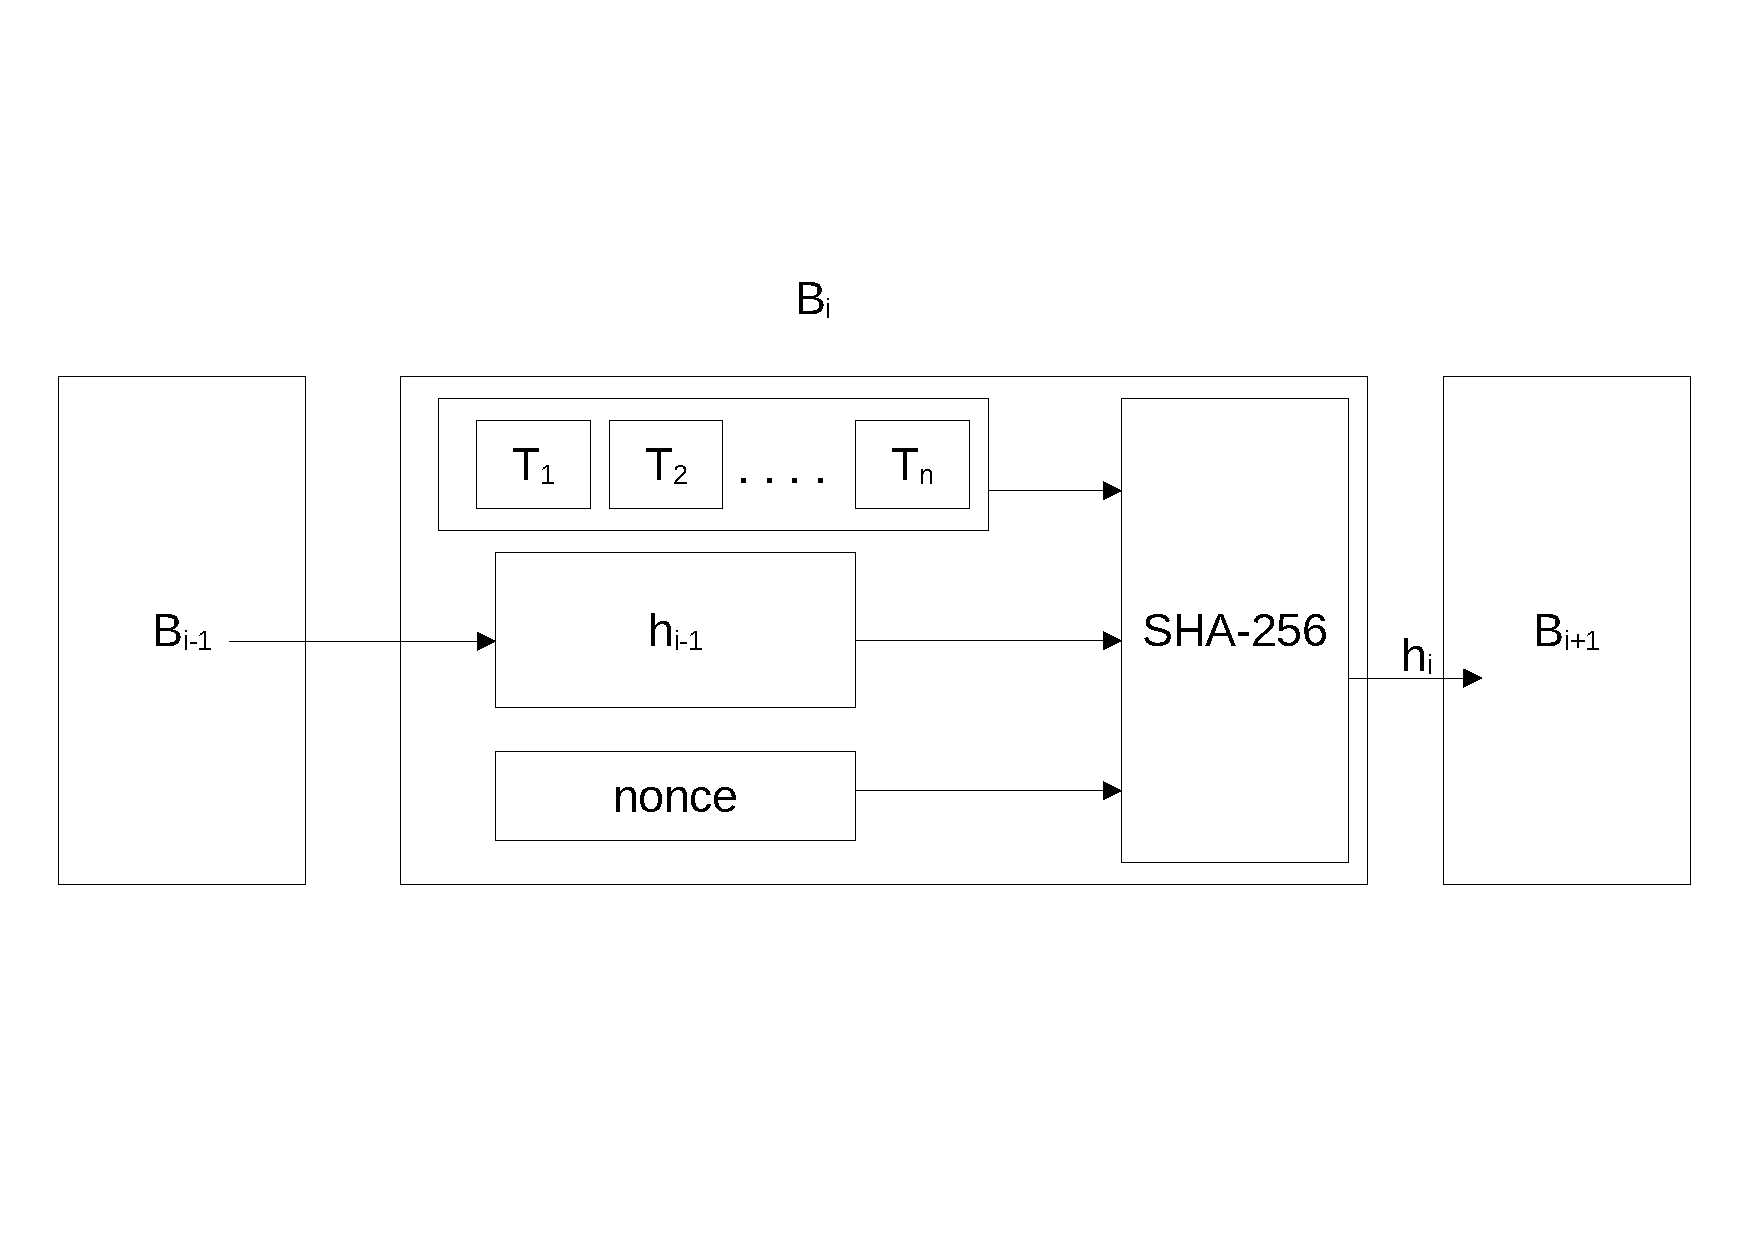
\includegraphics[scale=0.5, trim = 1cm 4cm 0cm 4cm, clip]{Images/blocchi_sha.pdf}
    \caption{Calcolo hash blocco $B_i$}
    \label{fig:sha-256}
\end{figure}
\FloatBarrier
Mentre le transazioni, e quindi anche la loro concatenazione, sono note nel blocco, così come è noto l’hash proveniente dal blocco precedente, il valore del nonce è incognito. L’attività di mining consiste nel risolvere un puzzle crittografico: trovare il valore del nonce tale che l’immagine hash prodotta dalla SHA-256 inizi esattamente con $t$ zeri, dove $t$ è un valore prefissato dal sistema, e variabile nel tempo.\\
La ricerca del nonce per la corretta aggiunta di un blocca è denominata \textbf{Proof of work}. L'unico modo per di trovare il nonce che produca un fingerprint che inizi con $t$ zeri, è quello di applicare ripetutamente la funzione SHA-256 con nonce via via diversi, finchè non si giunge ad un hash che soddisfa la proprietà desiderata. La risoluzione del problema è esponenziale in $t$, infatti la ricerca del nonce richiede tempo $O(2^t)$, ciò rende il problema di difficile risoluzione, in quanto è necessario far eseguire una lunga serie di calcoli alle macchine; nella pratica i calcolatori sono stati ottimizzati a livello hardware con lo scopo di calcolare il più rapidamente possibile la funzione SHA-256. Il valore di t viene aggiornato periodicamente dal sistema, in modo che la validazione di un blocco richieda sempre in media circa 10/15 minuti di tempo.\\Questo sistema evita che i blocchi già inseriti possano essere modificati retroattivamente: cambiando il contenuto di un blocco, ne cambierebbe anche il valore hash, e ciò implica il dover ricalcolare tutti i nonce dei blocchi successivi ad esso, perchè altrimenti le immagini hash non corrisponderebbero più tra blocchi consecutivi; dunque ciò che è stato scritto sulla blockchain è da considerarsi immutabile, a meno di rendere inconsistente tutta la struttura anche alterandone una sola transazione.\\I miner, ossia i nodi della rete che dispongono di calcolatori potenti abbastanza da risolvere le Proof of Work, rappresentano di fatto gli unici a poter avere il diritto di aggiungere transazioni alla blockchain, e nel farlo consumano un gran quantitativo di energia e di risorse di calcolo; per questo, il primo nodo di mining che riesce ad agganciare correttamente un blocco alla blockchain riceve un premio in bitcoin, nella forma di una transazione priva di input e con output l’address del miner: la \textbf{coinbase}, registrata anch’essa nella blockchain come una normale transazione. Il premio, di 25 bitcoin nel 2014, sarà dimezzato approssimativamente ogni quattro anni per essere definitivamente azzerato nel 2140 quando il numero complessivo di bitcoin esistenti dovrebbe raggiungere 21 milioni.
\section{Transazioni e Address in Bitcoin}
In questo  paragrafo verranno approfonditi i concetti stessi di transazione e di address, descrivendo con un grado di dettaglio funzionale ai nostri scopi il protocollo di pagamento e, anche in questo caso, la crittografia che vi sta dietro, sia per la diffusione delle transazioni che per la cifratura degli address.\\I software cliente di bitcoin, per esempio Bitcoin Core,, sono caricato sul PC o sullo smartphone di ogni utente A e genera anzitutto una coppia di chiavi privata-pubblica $k_A [prv]$, $k_A [pub]$ per un cifrario asimmetrico su curve ellittiche. La
chiave privata $k_A [prv]$ è ovviamente nota solo ad A e, come vedremo in seguito, è utilizzata da esso per firmare le transazioni che genera e diffonde sulla rete. La chiave pubblica $k_A [pub]$ è utilizzata per controllare la firma di A ed è anche impiegata come suo identificatore: a tale scopo viene trasformata attraverso applicazioni ripetute della funzione hash SHA-256 (immagine a 256 bit), per essere poi compressa via RIPEMD-160 in un’immagine di 160 bit in testa alla quale è aggiunta una speciale sequenza che indica che la stringa complessiva è di fatto un indirizzo bitcoin.
\begin{figure}[h!]
    \centering
    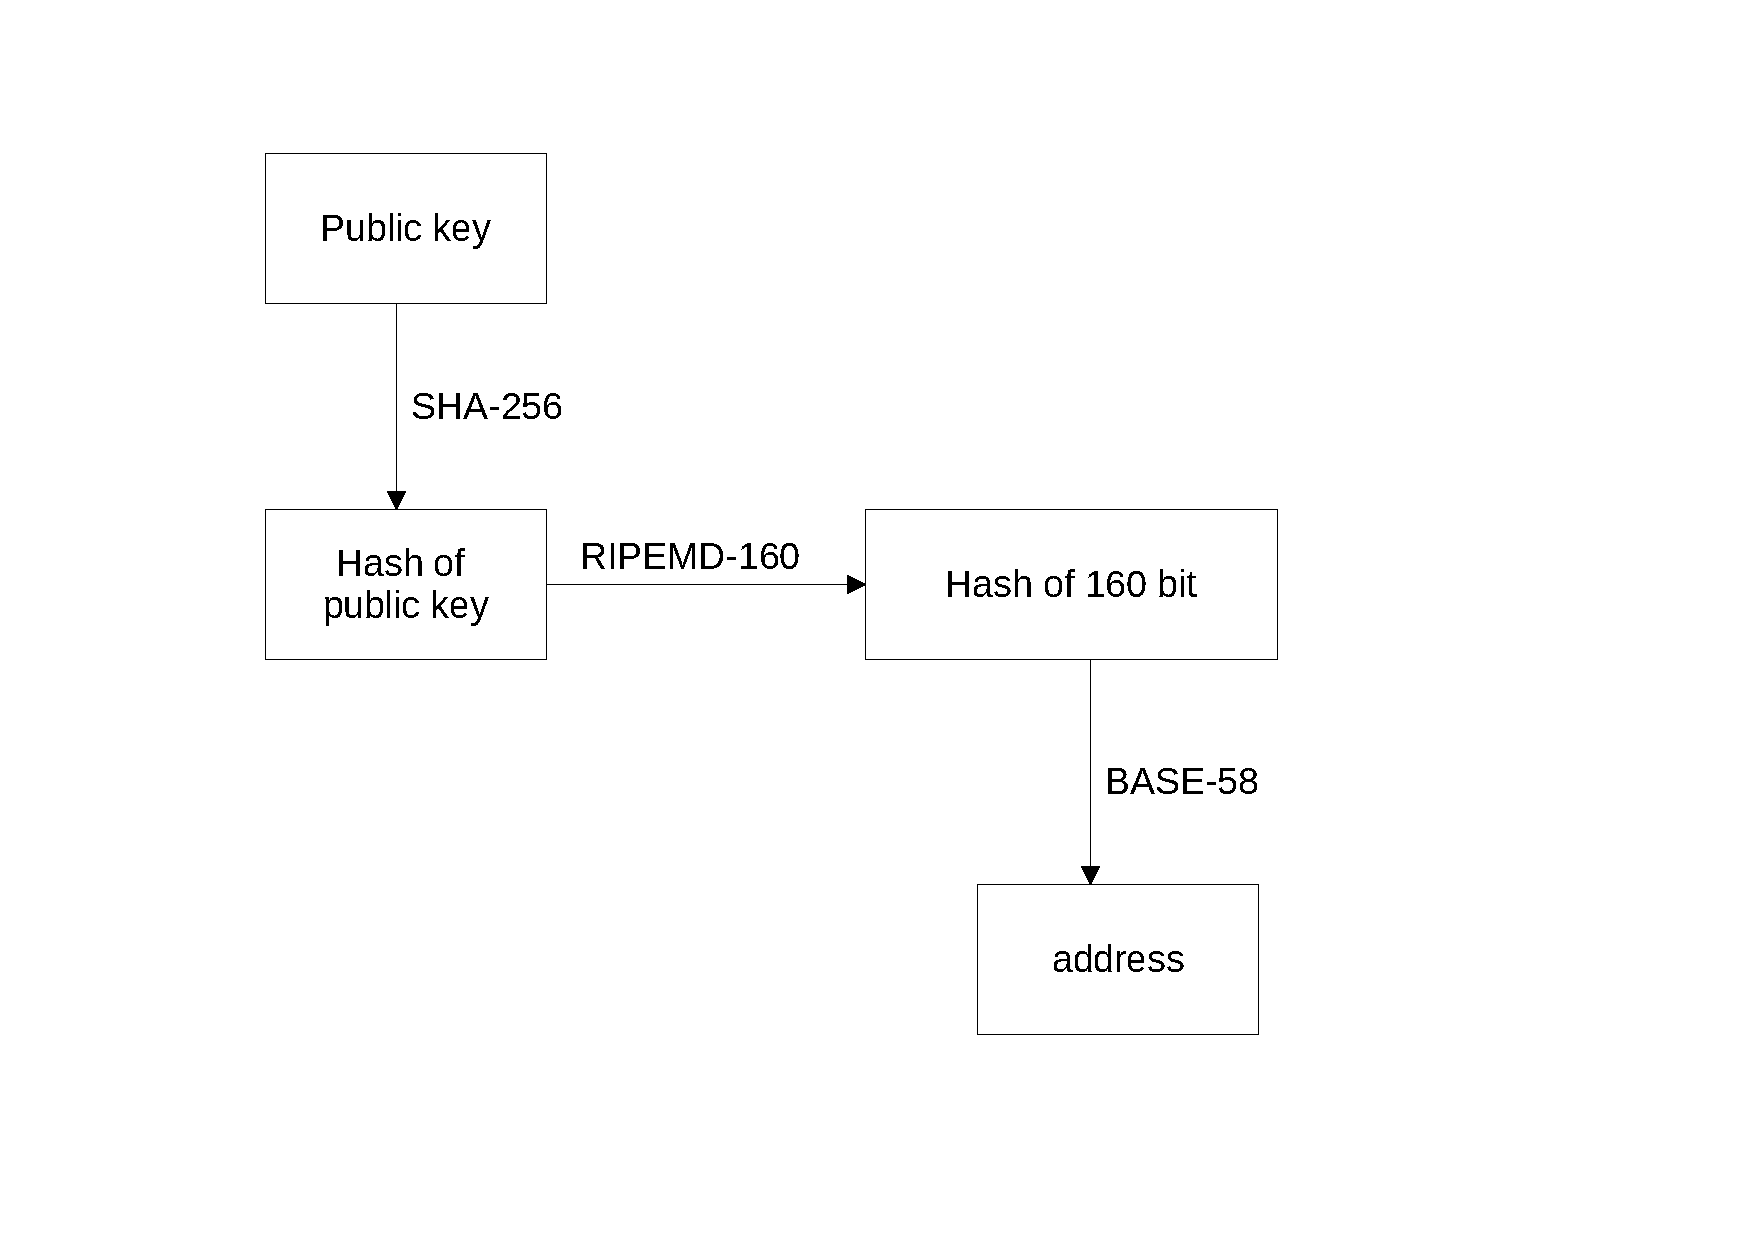
\includegraphics[scale=0.5, trim = 1cm 2cm 0cm 2cm, clip]{Images/address_gen.pdf}
    \caption{Generazione address in Bitcoin}
    \label{fig:sha-256_address}
\end{figure}
\FloatBarrier
Gli address in Bitcoin si presentano come stringhe alfanumeriche di questo tipo: 1BAFWQhH9pNkz3mZDQ1tWrtKkSHVCkc3fV.\\Come già osservato questo indirizzo non corrisponde a una “locazione” dell'utente ma a un modo per identificarlo, sia per potergli dirigere una transazione che per controllare che possieda effettivamente i fondi che pretende di spendere. Oltre a creare le chiavi e gli indirizzi il software cliente permette di costruire le transazioni. L'insieme delle coppie chiave pubblica-privata è contenuto all'interno di un apposito wallet, ad ognuna di queste coppie è associata un indirizzo però nessuno è a conoscenza del fatto che questi indirizzi appartengano allo stesso wallet. Questo è importante perchè così è possibile tracciare l'attività dei singoli address ma non l'attività di un intero wallet, garantendo un maggiore anonimato. Una transazione in bitcoin ha la forma “il pagatore A vuole inviare X bitcoin al ricevente B”, completata dalla firma digitale di A. Si noti che A e B sono indicati attraverso i loro indirizzi bitcoin e la transazione viene inviata per broadcast a tutti gli utenti. Diversamente da ogni altra forma di transazione economica, il ricevente B non ha la garanzia che la transazione sia valida finché, come vedremo, essa non è convalidata dalla rete. In effetti B sarebbe in grado di verificare sia la firma di A che i fondi che A ha a disposizione, poiché la chiave pubblica di A è nota e tutte le transazioni eseguite sulla rete sono pubbliche, ma non ha il tempo di verificare che A non abbia utilizzato gli stessi fondi in istanti immediatamente precedenti per pagamenti diversi. Formalmente una transazione è innescata secondo il seguente schema:
\begin{center}
\textbf{Protocollo di transazione Bitcoin}:
\begin{enumerate}
    \item L’utente A genera un messaggio m = $adr_A$ $-$ X $-$ $adr_B$ , dove $adr_A$ , $adr_B$ sono gli indirizzi Bitcoin di A e B, e X è la somma da trasferire da A a B.
    \item L’utente A calcola l’hash $h = SHA-256(m)$ del messaggio e genera la firma $f = D(h, k_A [prv])$ per m.
    \item La coppia $<m, f>$ viene diffusa in broadcast da A sulla rete.
    \item L’utente B attende che la rete convalidi la transazione prima di accettarla.
\end{enumerate}
\end{center}
La chiave privata è l’unico documento valido per dimostrare la proprietà in bitcoin di un utente A.
La perdita della chiave comporta la perdita della proprietà a causa dell’impossibilità di firmare transazioni, e il furto della chiave da parte di un truffatore che la usi per firmare al posto di A comporta anch’esso la perdita di proprietà.\\Un address acquisisce valore in base a quanti bitcoin detiene; quando si usa un address per pagare bitcoin (come input di una transazione), il suo valore viene azzerato, non è possibile spendere solo parte dei bitcoin che costituiscono il valore dell’address. Se un address A paga X bitcoin ad un address B, dopo la transazione il valore di A sarà azzerato, mentre il valore di B aumenterà di X bitcoin. In caso di eventuale resto, nel wallet del pagante si creerà un \textbf{change address}, che acquisirà un valore pari al resto ricevuto. Il change address può essere un address diverso da A, oppure A stesso, a discrezione dell’utente: per rafforzare l’anonimato è estremamente consigliabile da parte del pagante, al fine di ricevere i resti, utilizzare sempre address diversi da quelli usati per effettuare il pagamento.
\begin{figure}[h!]
    \centering
    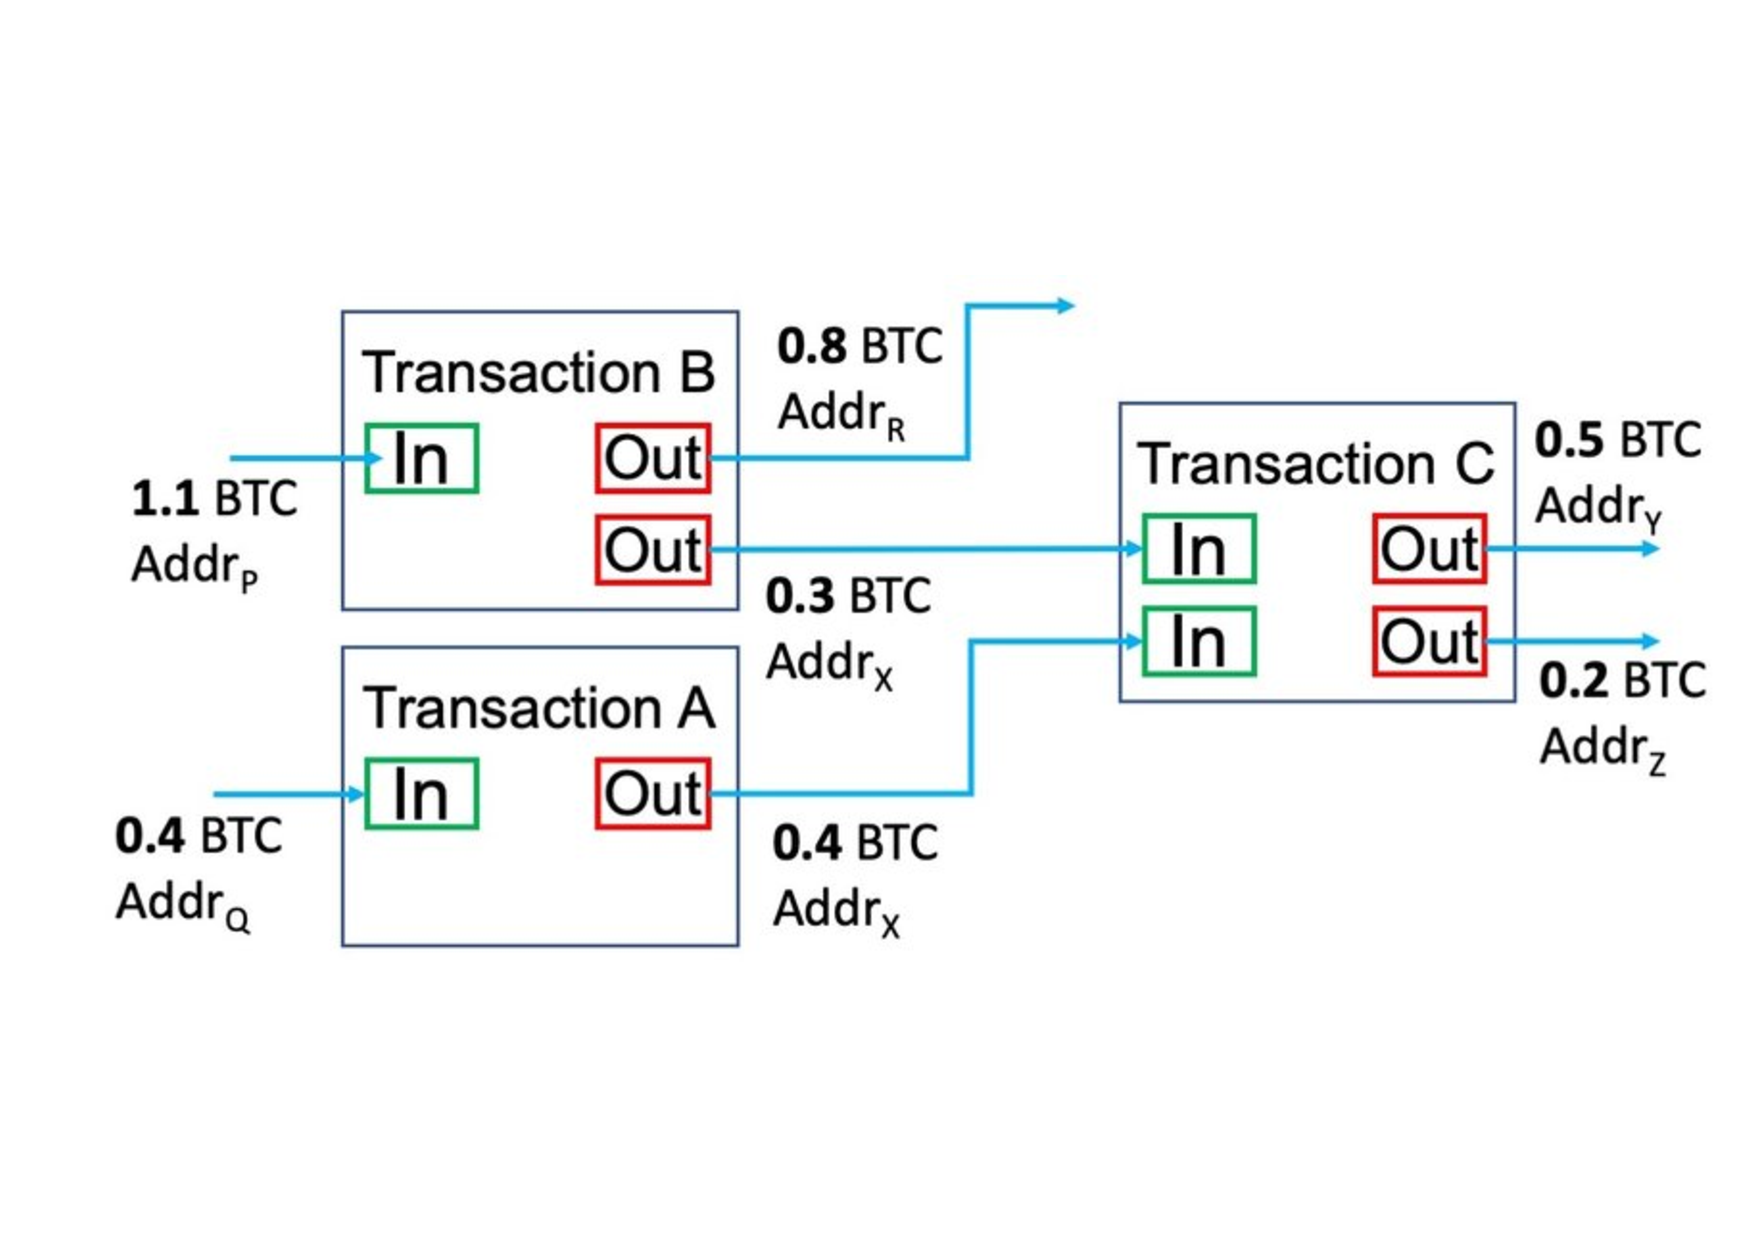
\includegraphics[scale=0.4, trim = 1cm 2cm 0cm 3cm, clip]{Images/Transactions-input-and-output-in-blockchain.jpg.pdf}
    \caption{Schema transazioni in Bitcoin}
    \label{fig:transaction}
\end{figure}
\FloatBarrier
Una transazione in generale può essere multi-input e multi output: sono presenti quindi più address paganti e/o più address riceventi, generalmente l'importo totale di input non viene speso in output ma parte di esso viene dato ai miners come fee. Formalmente la fee, raccolta dai miners come ricompensa per includere la transazione in un blocco, è definita come:
\begin{center}
    $fee = \sum_{inputs} importo(input_i) - \sum_{outputs} importo(output_i)$
\end{center}
Le transazioni in realtà sono molto più complesse di come le ho descritte precedentemente, non contengono solo valori come address e importo ma includono anche del codice, in particolare ogni transazione comprende anche degli script. Bitcoin utilizza un sistema di script Forth-like, basato su stack e non Turing-completo; questa scelta di evitare i loop è intenzionale in quanto impedisce possibili cicli infiniti.
\section{Anonimato in Bitcoin}



\chapter{Il Dust Attack}
Tra i molteplici attacchi all'anonimato di Bitcoin, un attacco interessante é il Dust Attack, chiamato anche ``Forced reuse address" \cite{dst_att_def}. Il Dust Attack é una nota tecnica di de-anonimizzazione il cui obiettivo é capire che certi address appartengano al medesimo wallet.

In questa tesi:
\begin{itemize}
\item Definiremo il concetto di dust;
    \item Presenteremo le modalità più comuni con cui viene speso il dust, in particolare analizzeremo se e quanto possa essere efficace un Dust Attack mostrando gli effetti del dust sulla de-anonimizzazione degli address e dei relativi wallet;
    \item Descriveremo alcuni pattern interessanti che sono stati individuati e che potrebbero essere messi in relazione con il  Dust Attack.
\end{itemize}

Poiché il Dust Attack sfrutta l'utilizzo degli importi dust, é importante quindi spiegare cosa sia il dust e in generale quali possano essere i suoi possibili impieghi.

\section{Definizione del dust}
Il dust é una piccola quantità di criptovaluta presente in un UTXO sotto i limiti minimi di scambio, che chiariremo in seguito. Per definire il valore del dust é necessario fare alcune considerazioni.

Nelle transazioni di Bitcoin, generalmente, l'importo totale di input non viene speso completamente in output ma parte di esso viene inviato ai miners come fee. Formalmente la fee di una transazione, raccolta dai miners come ricompensa per includere la transazione in un blocco, é definita come:
\begin{center}
    $fee = \sum_{i=0}^{\#inputs} importo(input_i) - \sum_{j=0}^{\#outputs} importo(output_j)$
\end{center}
La fee quindi non é altro che la differenza tra l'importo totale di input e l'importo totale di output, e assume valori $\ge 0$. In generale la fee viene stabilita autonomamente dal creatore della transazione per incentivare i miners a validare la transazione stessa. Più la fee scelta é proporzionalmente alta, e più i miner guadagneranno nel validare la relativa transazione, rendendo la transazione prioritaria e quindi validata più in fretta.

Tuttavia, per convenzione, esiste una fee minima, denominata \textit{minimum relay fee}, che una transazione si suppone pagare affinché un qualsiasi nodo della rete peer-to-peer inoltri quella transazione agli altri nodi della rete. Questo valore non é prefissato ma varia piuttosto nel tempo in base allo stato della rete e all'andamento del suo valore. 

Nella comunità Bitcoin, spesso nuove convenzioni e comportamenti suggeriti sono pubblicati attraverso il client ufficiale, Bitcoin Core \cite{btccore}, poiché rimane ancora oggi il client più diffuso nella rete.  Tale client ha introdotto una convenzione, definita ``dust limit", che va rispettata per mantenere lo stato di transazione standard, cioé quelle transazioni che i nodi sono suggeriti accettare ed inoltrare ad altri nodi.

Lo scopo é quello di considerare non-standard le transazioni che includono degli output dust proprio perché costerebbe di più per il destinatario spendere l'importo dust rispetto al valore dell'output creato. Infatti un importo dust non può essere speso da solo in una transazione standard, poiché minore della \textit{minimum relay fee}, perciò deve essere necessariamente aggregato ad altri input.

In generale un valore dust consuma in fees un valore maggiore di quello scambiato. Questo di fatto lo rende razionalmente non spendibile, poiché il destinatario dovrebbe spendere più di quanto riceverebbe per ottenerlo. L'output però rimane tecnicamente spendibile e quindi deve essere mantenuto nell'UTXO, appesantendo inutilmente la struttura dati con valori inutili.

Il limite attuale é di 546 satoshi \cite{BtcDev}. Quindi tutti gli importi minori di 546 satoshi sono definiti \textbf{dust}.

\section{Possibili utilizzi del dust}

Gli usi del dust possono essere molteplici. Per esempio può essere utilizzato per effettuare degli stress test della rete Bitcoin, proprio perché permette di generare tante transazioni con molti output ad un basso costo complessivo. In questo caso il costo é determinato principalmente dalla fee della transazione e non tanto dagli output. Se consideriamo che il valore di 1 satoshi, unità minima di Bitcoin, vale meno di due centesimi di euro al momento (Novembre 2022), é possibile generare una transazione con 1000 output dust, 1 satoshi ciascuno, con meno di venti centesimi (fee esclusa).

In generale, dato l'irrilevante valore economico del dust, viene spesso usato per ottenere effetti laterali, diversi dal semplice scambio di valore. Nel seguito mostriamo tre esempi interessanti di tale uso del dust: la notifica dell'esito di scommesse nel servizio di gambling Satoshi Dice, la scrittura di dati arbitrari tramite lo script OP\_RETURN ed il Dust Attack.

\subsection{Satoshi Dice}
Satoshi Dice é un noto ``gioco di scommesse basato su blockchain" nato nell'Aprile 2012 \cite{SD}. A differenza dei tradizionali software di gioco online, le scommesse con Satoshi Dice possono essere inviate senza accedere ad un sito Web né eseguire alcun software client. Per giocare, viene effettuata una transazione Bitcoin a uno degli address resi pubblici da Satoshi Dice, caratterizzato da probabilità di vincita e quindi di pagamenti diversi.

Per essere meglio riconoscibili, tutti gli address resi pubblici da Satoshi Dice sono \emph{vanity address}. Un vanity address é un normale address Bitcoin con le stesse funzionalità di qualsiasi altro address ma inizia con una stringa alfanumerica personalizzata contenente una parola o un messaggio comprensibili alle persone. Un esempio di vanity address é \textit{1SochiWwFFySPjQoi2biVftXn8NRPCSQC}, che contiene la parola Sochi, città in cui si sono svolte le olimpiadi invernali nel 2014. Tutti gli address di Satoshi Dice presentano infatti il prefisso \textbf{1dice}.

Ogni address ha associate probabilità diverse di vincere la scommessa, generalmente minore é la probabilità maggiore é il compenso che si ottiene da una vincita. Per esempio l'address \textit{1dice1e6pdhLzzWQq7yMidf6j8eAg7pkY} offre una probabilità dello 0,0015\% di vincere 64 000 volte la puntata originale.

Per determinare se una scommessa é vincente o perdente, Satoshi Dice genera un numero pseudo casuale, il quale viene assegnato al giocatore. Per ottenere tale numero, il servizio utilizza una combinazione dell'hash della transazione della scommessa ed esegue un hash SHA2 a 256 bit prendendo come input l'hash della transazione e un altro parametro sconosciuto al giocatore (un valore segreto giornaliero, pubblicato il giorno dopo per permetterne la verifica). I primi quattro byte dell'output diventano il numero che determina se il giocatore abbia vinto la scommessa.

Il servizio, dopo aver determinato le scommesse vincenti e quelle perdenti, invia una transazione in risposta con il pagamento ai vincitori e restituisce un singolo satoshi ai giocatori perdenti per comunicare loro la perdita. Questo significa che Satoshi Dice utilizza il dust, 1 satoshi, per comunicare la perdita di una scommessa. Nel periodo tra l'Aprile 2012 e Agosto 2017 Satoshi Dice ha generato più di un milione di transazioni in cui invia questi importi dust, a dimostrazione della popolarità raggiunta dal servizio.

\subsection{Dust in OP\_RETURN}
Le transazioni in Bitcoin a basso livello sono più complesse \cite{script} di come descritte nella precedente sezione \ref{Transazioni}. Non contengono, infatti, solo valori come address e importo ma includono anche del semplice codice. In particolare ogni transazione comprende anche degli script che descrivono quali siano le condizioni che devono essere verificate affinché il destinatario dei bitcoin possa spenderli. 

Bitcoin utilizza un sistema di script Forth-like, basato su stack e non Turing-completo; questa scelta é intenzionale in quanto impedisce possibili cicli infiniti. Gli script in Bitcoin sono \cite{opcode}:
\begin{itemize}
    \item Senza stato: non esiste uno stato prima dell'esecuzione di uno script né lo stato viene salvato dopo l'esecuzione.
    \item Deterministici: uno script viene eseguito alla stessa maniera in ogni nodo.
    \item Semplici e compatti: le istruzioni, gli OP\_CODE, sono codificate in un singolo byte. In totale ci sono 75 istruzioni funzionanti e 15 disabilitate.
\end{itemize}
Gli OP\_CODE in Bitcoin comprendono diverse categorie:
\begin{itemize}
    \item aritmetica di base: OP\_ADD, OP\_SUB;
    \item controllo di flusso: OP\_IF, OP\_ELSE;
    \item logica bit a bit: OP\_EQUAL;
    \item gestione stack: OP\_DROP, OP\_SWAP;
    \item hashing: OP\_SHA1, OP\_SHA256;
    \item verifica firma o multifirma: OP\_CHECKMULTISIG.
\end{itemize}

Le transazioni Bitcoin non forniscono un campo dove si possono salvare dati arbitrari \cite{arbdata}. Tuttavia, gli utenti hanno ideato diversi modi creativi per codificare dati arbitrari nelle transazioni, in particolare memorizzando valori arbitrari negli output delle transazioni. Questi metodi però modificavano il protocollo rendendo non spendibili gli output così generati. Il problema é che questi output artefatti non sono facilmente distinguibili dagli altri quindi i nodi della rete devono salvarli comunque nei loro UTXO.
Poiché questo set, per motivi di efficienza, é solitamente memorizzato nella RAM \cite{utxo} questa pratica influisce negativamente sul consumo di memoria dei nodi \cite{stresstest}.

Per risolvere tale problema a partire dal 2014 é stato reso standard il codice OP\_RETURN \cite{opreturnstandard}. Questo OP\_CODE era presente fin dalla nascita di Bitcoin e permette di segnare un output della transazione come non valido, quindi successivamente non potrà essere speso. Questo però era considerato uno script non-standard proprio perché la scrittura di dati arbitrari sulla blockchain non é stata considerata fin dall'inizio una buona pratica.

Poiché gli output con questo OP\_CODE sono contrassegnati come non spendibili, possono essere rimossi dall'UTXO set. In questo modo OP\_RETURN risolve il problema del consumo di memoria spiegato precedentemente. Il limite iniziale per la memorizzazione dei dati con questo codice era pianificato essere di 80 byte, ma inizialmente ne furono concessi 40 (versione 0.9.0).  La versione 0.11.0 \cite{v11} ha esteso il limite di dati a 80 byte e la versione 0.12.0 \cite{v12} fino a un massimo di 83 byte. Inoltre una transazione standard non può contenere più di un output contenenti OP\_RETURN, la figura \ref{opreturnn} mostra un esempio di un output generato con questo script.
\begin{figure}[h!]
    \centering
    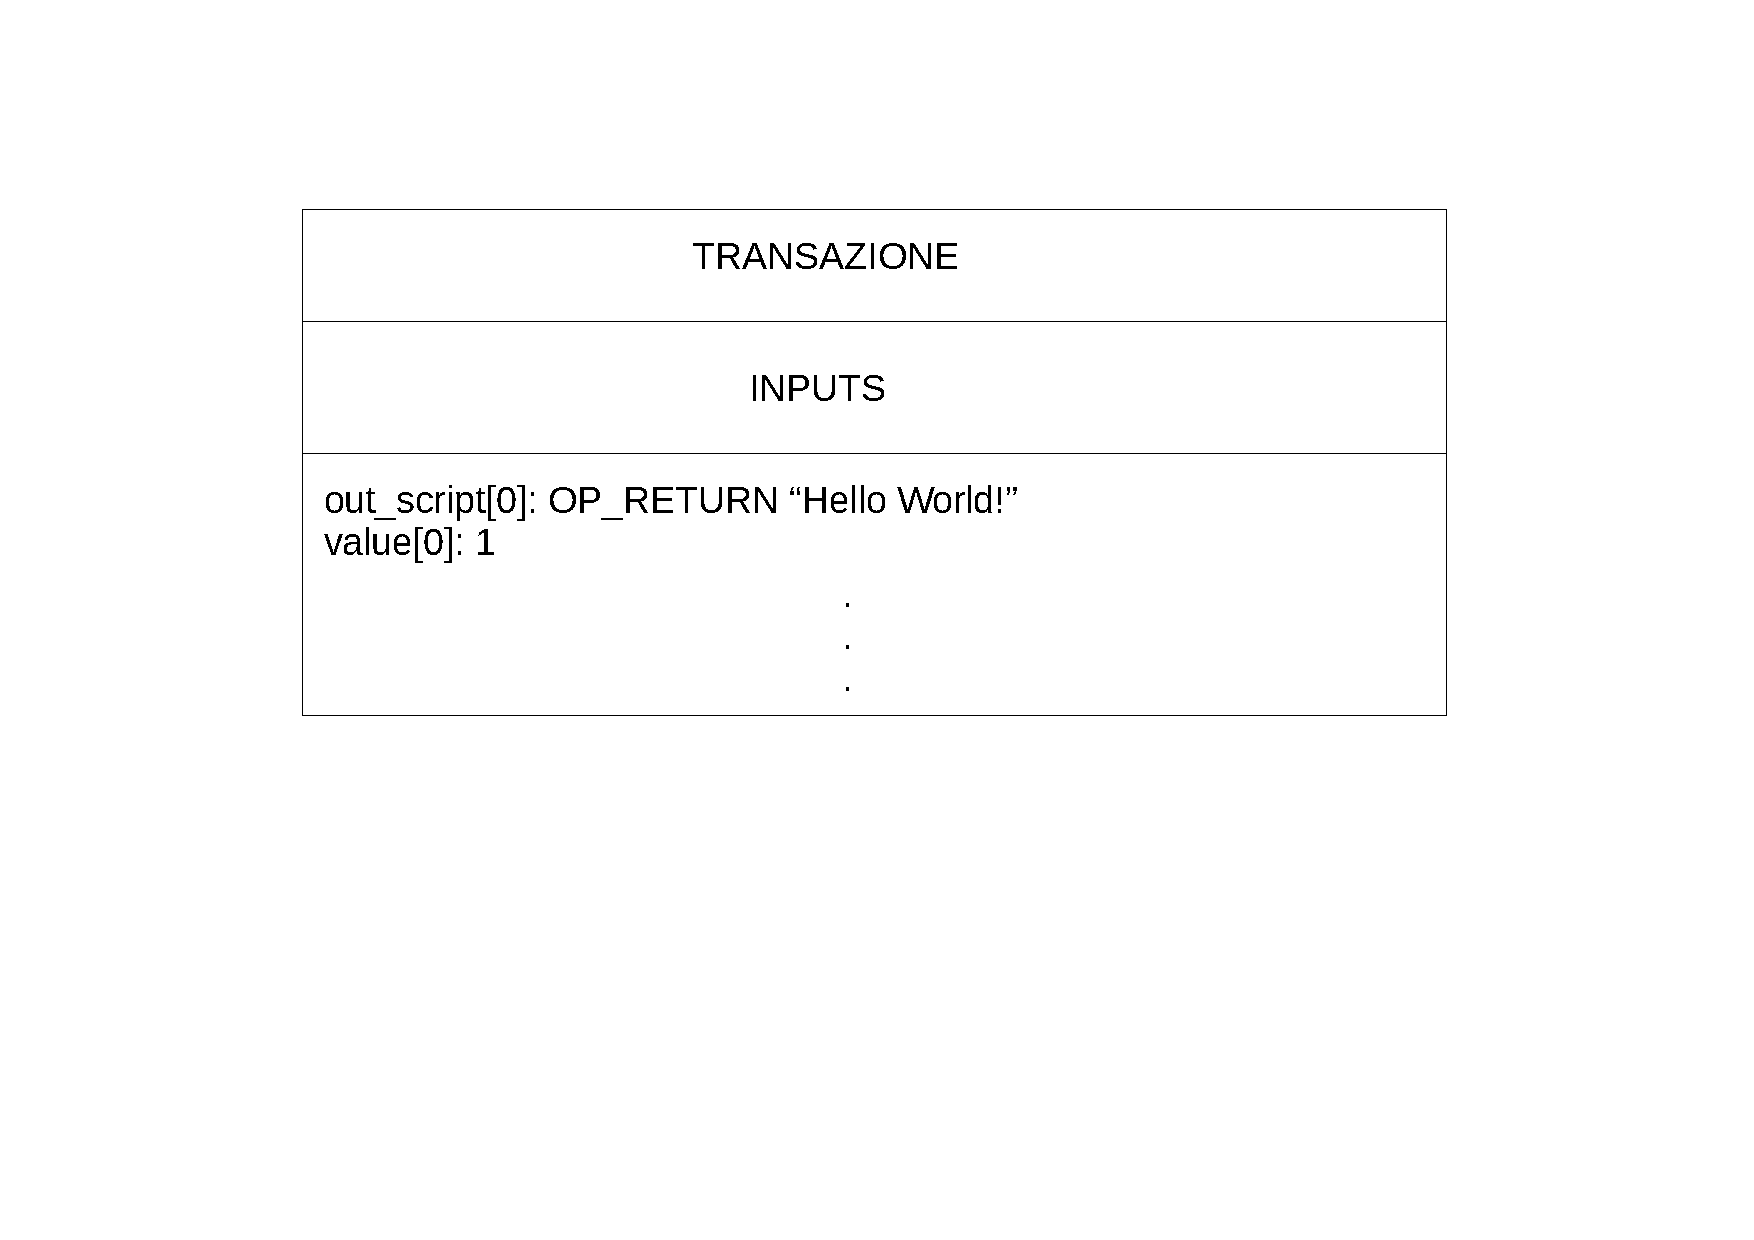
\includegraphics[scale=0.5, trim = 1cm 8cm 0cm 3cm, clip]{Images/opreturnn.pdf}
    \caption{Esempio di output con OP\_RETURN}
    \label{fig:opreturnn}
\end{figure}
\FloatBarrier

Poiché per scrivere dati arbitrari sulla blockchain é comunque necessario generare una transazione con almeno un output risulta quindi molto più conveniente generare output con importi dust per ridurre al minimo i costi della transazione.

Come riportato in \cite{OP_RETURN} esistono diversi protocolli che sfruttano OP\_RETURN. Di solito, un protocollo é identificato dai primi byte di metadati allegati all'OP RETURN, ma il numero esatto di byte può variare da protocollo a protocollo. 

Questi protocolli possono essere divisi in diverse categorie come ad esempio:
\begin{itemize}
    \item \textbf{Risorse}: protocolli che sfruttano l'immutabilità della blockchain per certificare la proprietà, lo scambio e, infine, il valore dei beni del mondo reale. I metadati nelle transazioni vengono utilizzati per specificare ad es. il valore del bene, l'importo del bene trasferito, il nuovo proprietario, ecc;  
    \item \textbf{Atti notarili}: protocolli per la certificazione della proprietà di un documento. Un utente può pubblicare l'hash di un documento in una transazione, e in questo modo può provarne l'esistenza e l'integrità;
    \item \textbf{Arte digitale}: protocolli per la dichiarazione dei diritti di accesso e di copia di arti digitali, come ad es. foto o musica.
\end{itemize}

\section{Il Dust Attack}\label{dstatt}
Come analizzato nella precedente sezione \ref{Anonimato} esistono delle euristiche che possono essere sfruttate per effettuare determinati attacchi in grado di violare l'anonimato di Bitcoin. L'attacco che verrà approfondito in questa tesi viene denominato \textbf{Dust Attack}. 

L'euristica utilizzata da questo tipo di attacco é la regola degli input multipli:
\begin{center}
    ``\textit{In una transazione multi-input tutti gli address spesi negli input appartengono allo stesso utente}"
\end{center}
L'obiettivo del Dust Attack é la de-anonimizzazione del proprietario di un wallet, in particolare l'attaccante vuole scoprire quali address appartengano allo stesso wallet, così da ottenere un'importante informazione che può essere utilizzata per effettuare altri attacchi più elaborati e pericolosi.

Il Dust Attack deriva il proprio nome dall'impiego del dust, e si basa sulla regola che il dust, nelle transazioni standard, non può essere speso singolarmente ma deve sempre essere unito ad altri importi. L'attaccante quindi, come mostrato in figura \ref{fig:Dust_attack}, invia centinaia, o migliaia, di importi dust ad address diversi confidando che vengano spesi successivamente in una nuova transazione insieme ad altri address. Se ciò avviene l'attaccante riesce a collegare questi address e capire che appartengono, con una certa probabilità, allo stesso utente. Gli address a cui viene inviato il dust sono tutti address già comparsi in precedenza sulla blockchain. Infatti, le transazioni che inviano del dust ad address nuovi molto probabilmente non rappresentano un Dust Attack, proprio perché risulterebbe alquanto inusuale de-anonimizzare un address mai visto fino a quel momento. In generale un nuovo indirizzo é creato come change address dal creatore della transazione o come nuovo indirizzo di pagamento dal destinatario del pagamento. Nel caso di Dust Attack, molto probabilmente il proprietario di un address nuovo é lo stesso utente che genera quella determinata transazione poiché é l'unico a conoscenza di quel determinato address, quindi, nel nostro caso, l'attaccante stesso.

Il Dust Attack ad un primo sguardo potrebbe sembrare particolarmente costoso, proprio perché invia tanti importi ad address differenti, ma se analizziamo il valore in euro di un singolo satoshi, si può osservare che il costo é relativo; soprattutto se l'obiettivo finale é tentare un furto dei bitcoin delle vittime. Infatti abbiamo che:
\begin{center}
    1 satoshi = 0.00016 € (in data 16/11/2022) 
\end{center}

Questo significa che 1 singolo satoshi vale meno di 1 centesimo, quindi se un attaccante genera una transazione con 1000 output dust e manda a ciascun address 1 satoshi, in totale spende 16 centesimi, escludendo la fee.   
\begin{figure}[h!]
    \centering
    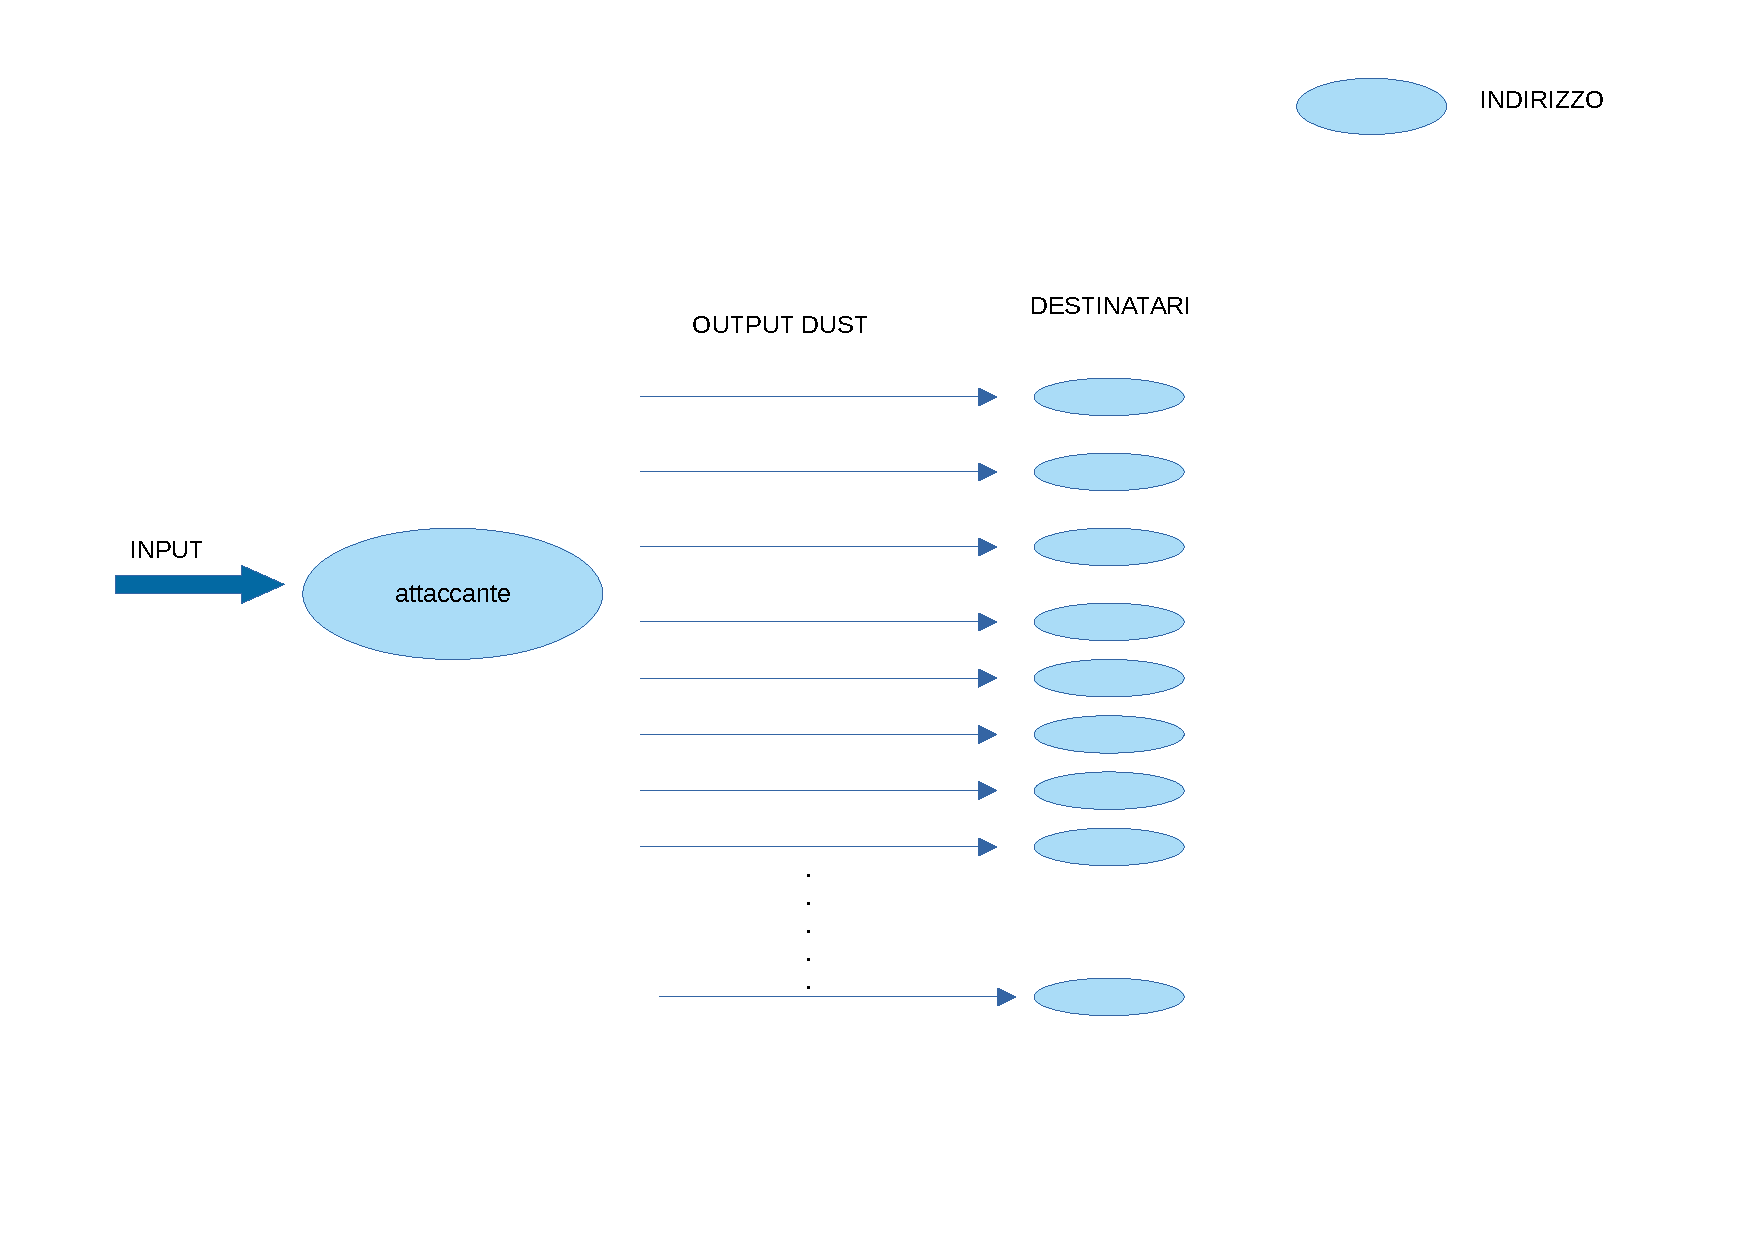
\includegraphics[scale=0.5, trim = 1cm 5cm 0cm 0cm, clip]{Images/dust_attack.pdf}
    \caption{Schema Dust Attack}
    \label{fig:Dust_attack}
\end{figure}
\FloatBarrier
Possono esserci due possibili esiti del Dust Attack: 
    \begin{enumerate}
        \item attacco di successo;
        \item attacco fallito.
    \end{enumerate}
    
Nel primo caso, mostrato in figura \ref{fig:success}, la vittima genera una transazione in cui spende l'importo dust ricevuto insieme ad almeno un altro dei suoi address. 

Questi address quindi sono collegati tra loro dalla euristica sui multi-input, ed é possibile capire che appartengano ad uno stesso utente. Se l'attaccante successivamente scopre le informazioni personali, come nome o email, del proprietario di uno di questi address automaticamente scopre che tutti gli altri address hanno lo stesso proprietario. Inoltre é possibile tracciare l'attività di un utente e non solo di un singolo address.
\begin{figure}[h!]
    \centering
    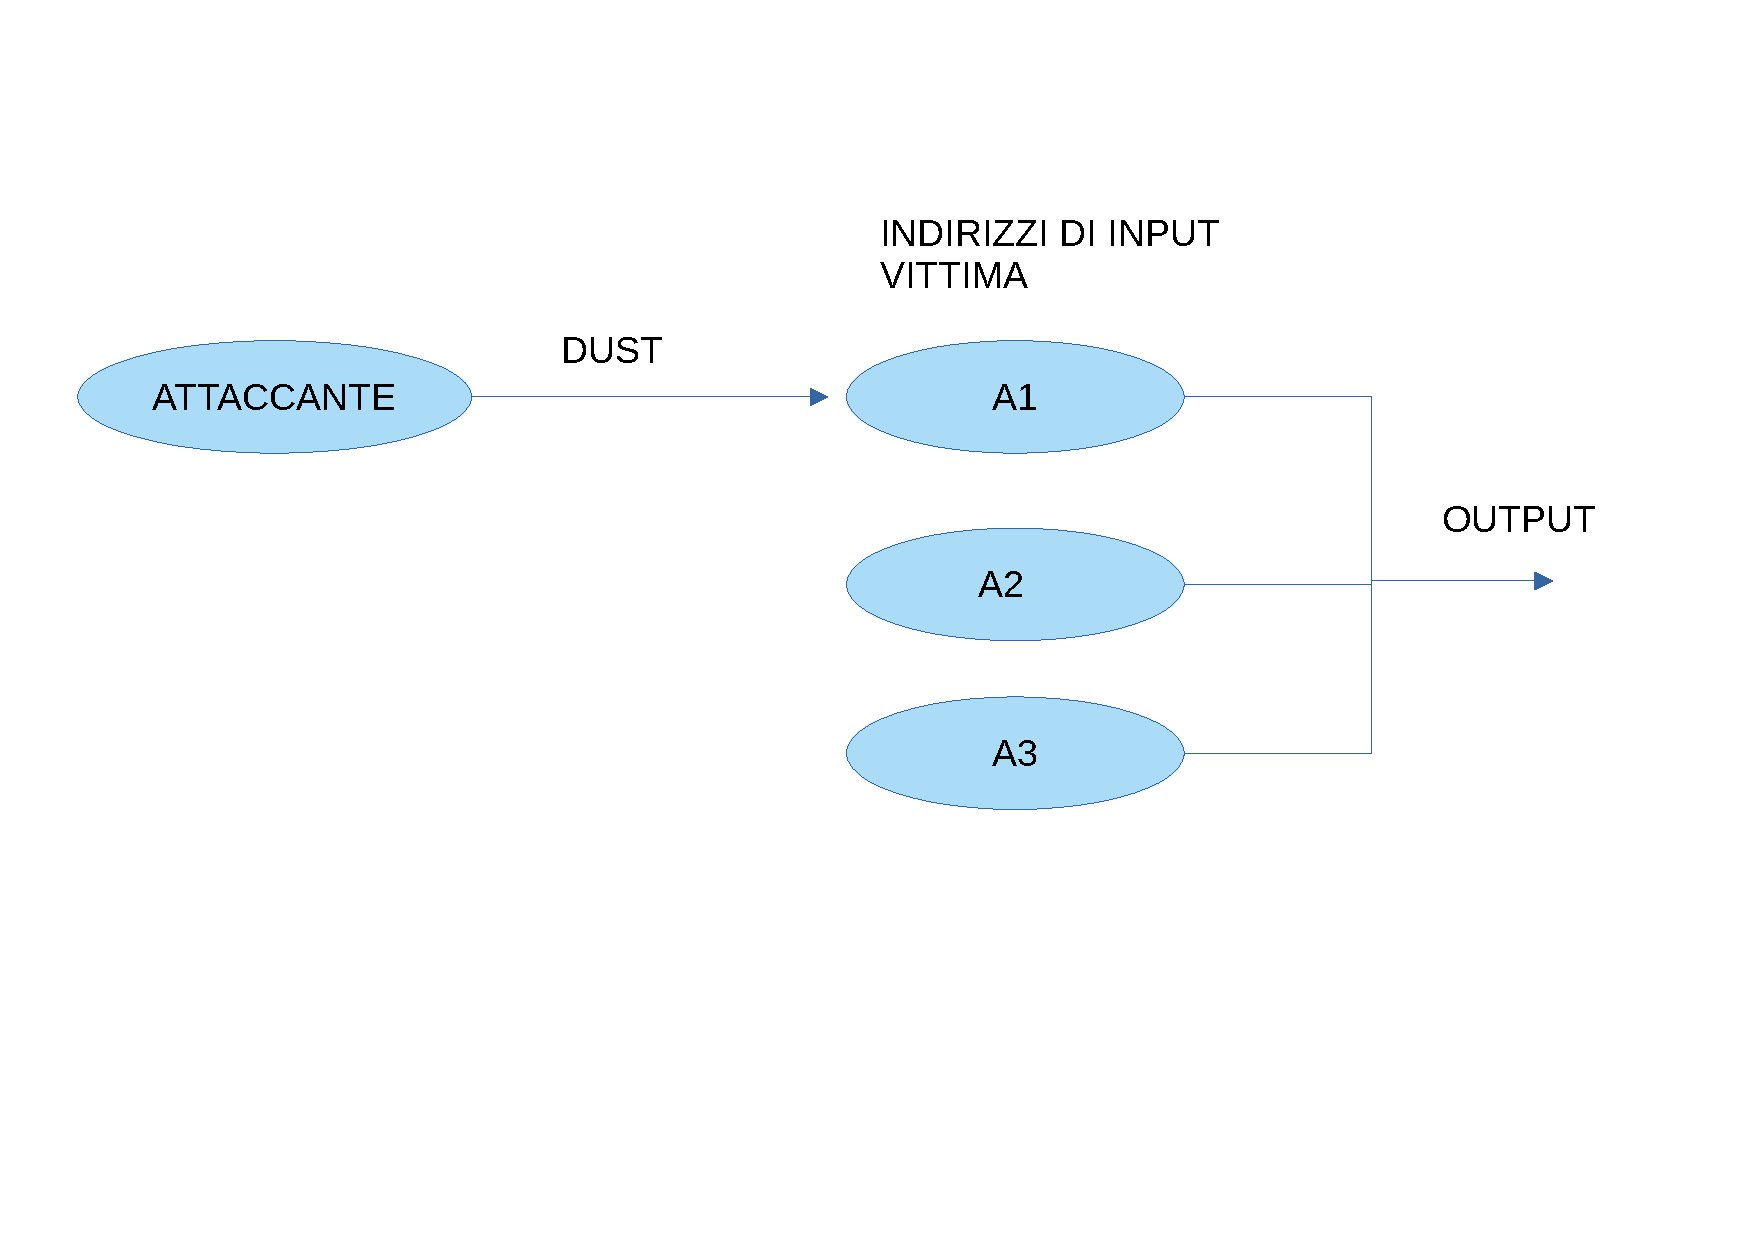
\includegraphics[scale=0.5,trim = 1cm 6cm 0cm 3cm, clip]{Images/successo.pdf}
    \caption{Schema di Dust Attack di Successo: l'address del dust viene speso con altri address}
    \label{fig:success}
\end{figure}
\FloatBarrier
Esistono invece due possibili motivi per cui un Dust Attack può fallire. In figura \ref{fig:fallito} vengono schematizzati questi due possibili esiti.

Nel primo schema la vittima spende il dust ricevuto, ma utilizza una transazione i cui input si riferiscono ad UXTO relativi all'address in cui é stato depositato il dust. In questo caso l'attaccante non ricava alcuna informazione perché non riesce nell'intento di provocare l'unione di address diversi di un utente nella medesima transazione. Nel secondo schema invece la vittima non spende il dust, troncando sul nascere l'attacco. 

Il Dust Attack, in generale, risulta più efficace soprattutto se il dust é diretto verso gli address che hanno un bilancio complessivo pari a zero proprio perché obbliga la vittima a spendere la cifra ottenuta con altri suoi address diversi.

\begin{figure}[h!]
    \centering
    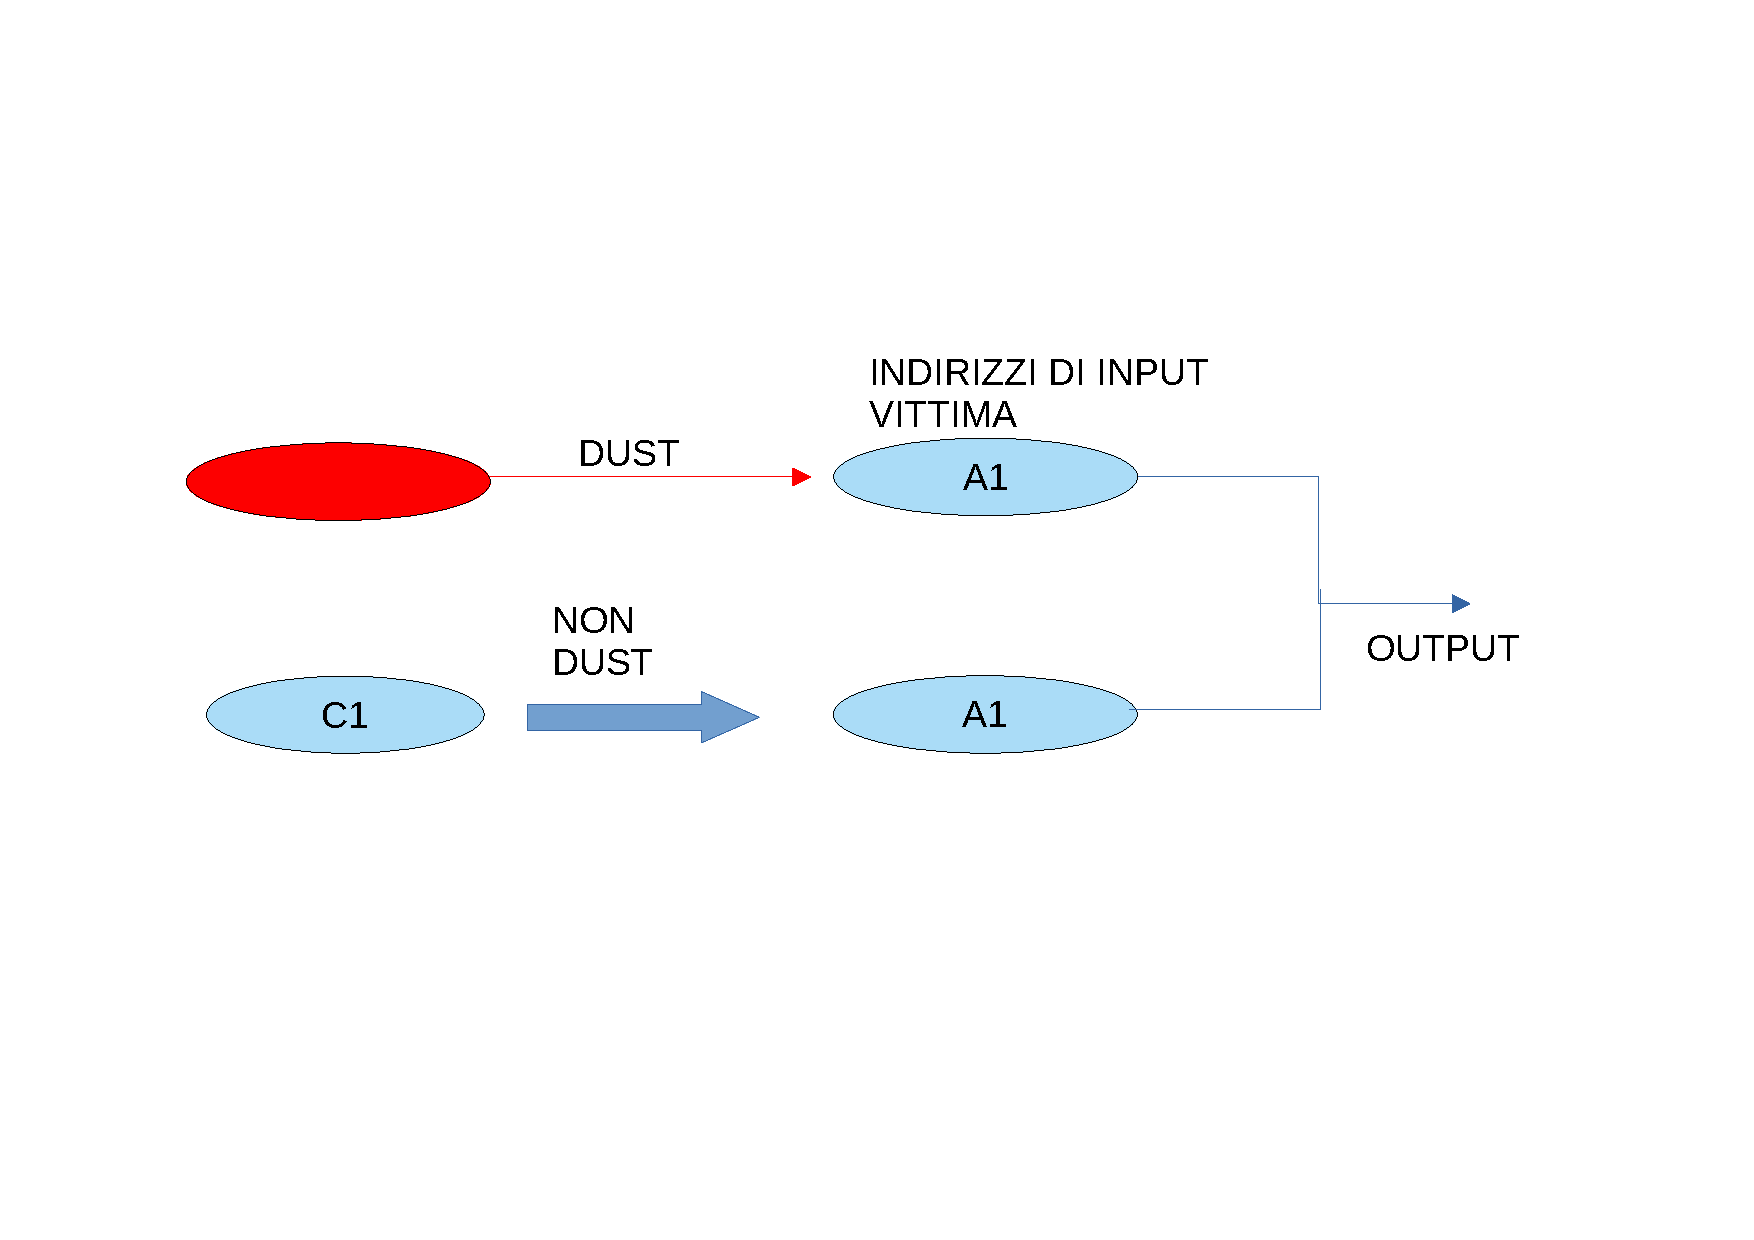
\includegraphics[scale=0.5, trim = 1cm 6cm 0cm 3cm, clip]{Images/fallito2.pdf}
    (a)
    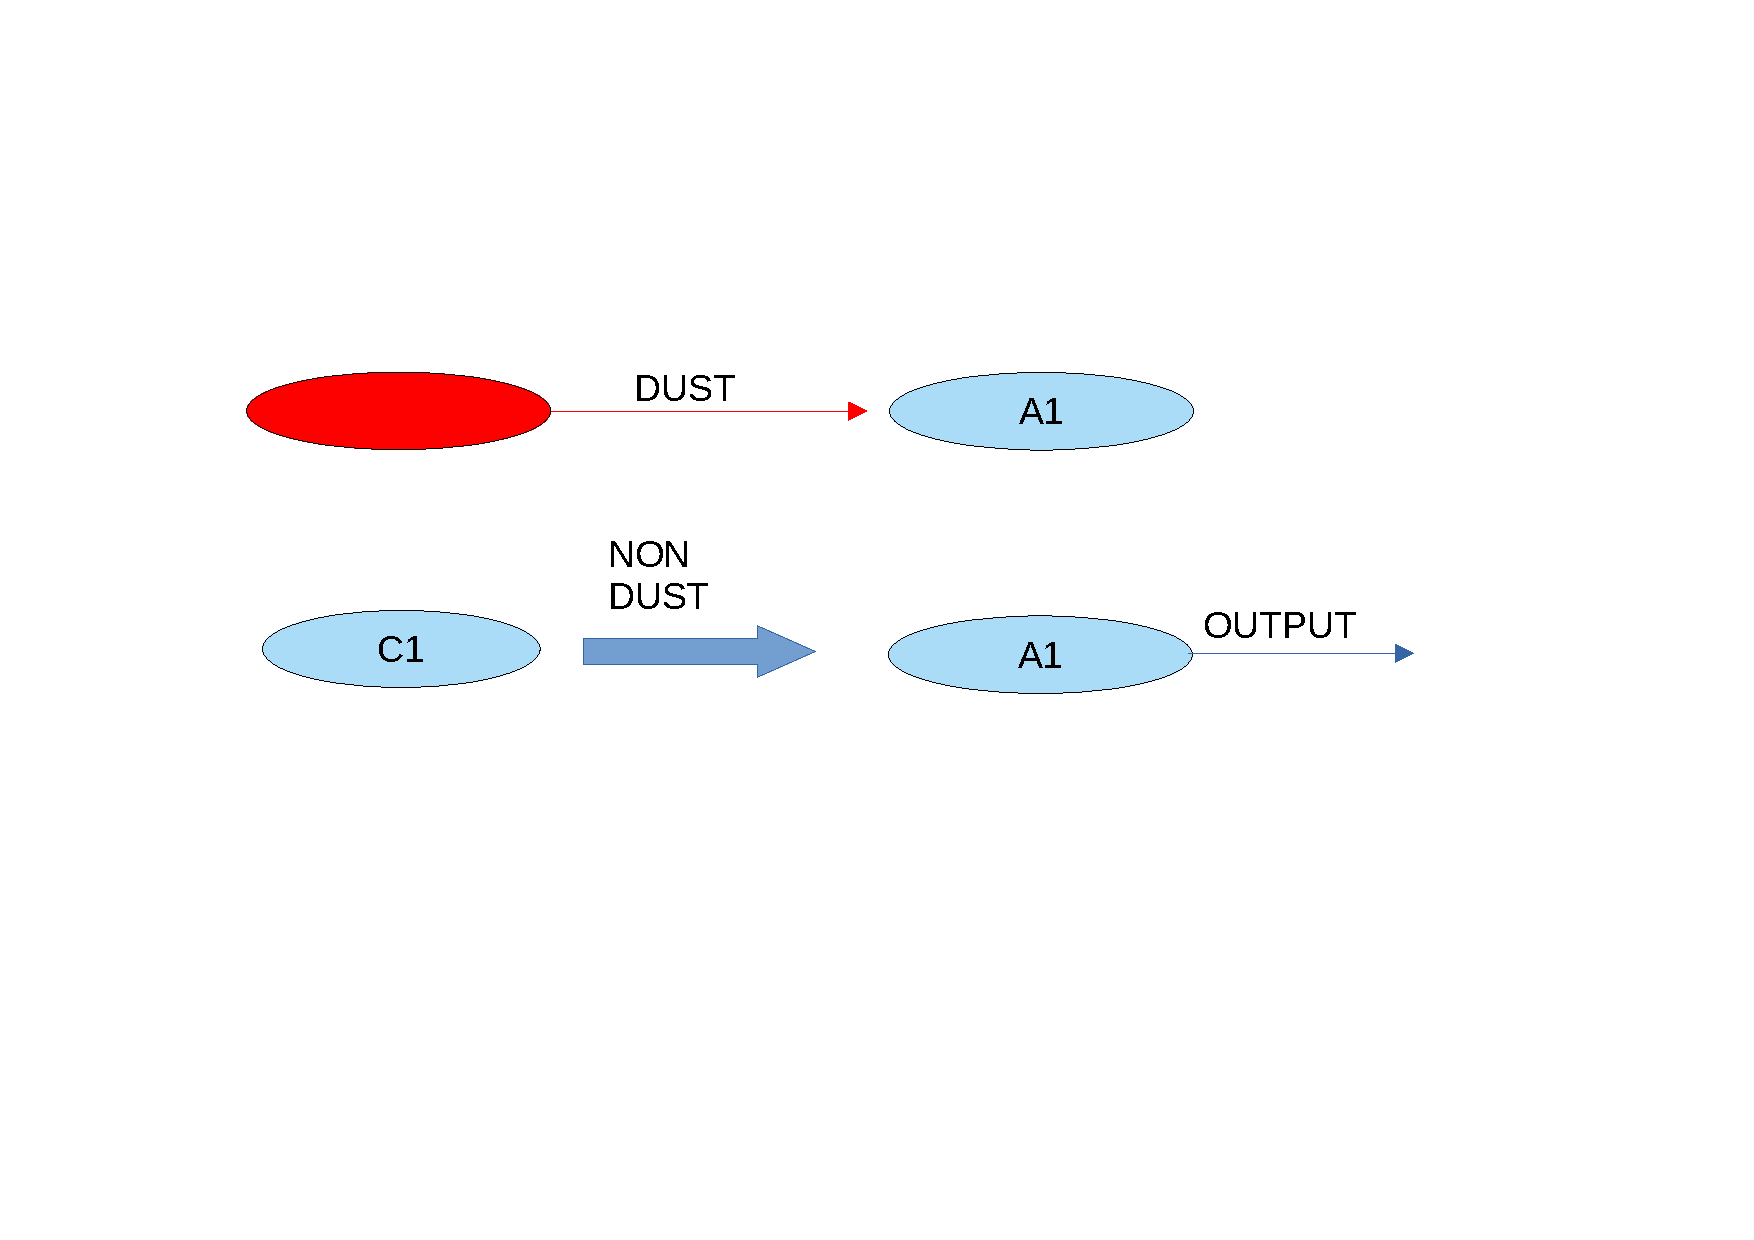
\includegraphics[scale=0.5, trim = 1cm 7cm 0cm 2cm, clip]{Images/fallito1.pdf}
    (b)
    \caption{Schema di Dust Attack Fallito. La vittima spende il dust con un solo address(a), la vittima non spende il dust(b)}
    \label{fig:fallito}
\end{figure}
\FloatBarrier

é importante notare che lo scopo del Dust Attack non é quello di rubare fondi di altri utenti né quello di scoprire informazioni personali, per esempio nome e cognome, della vittima. Permette, invece, di rompere lo pseudo-anonimato degli address, ovvero l'appartenenza di address differenti ad uno stesso utente. Questa informazione può essere usata in seguito per effettuare attacchi elaborati e più pericolosi.

In generale il Dust Attack non necessariamente é legato a phishing o estorsioni ma potrebbe essere usato dalle autorità per tenere traccia degli utenti ed eventualmente rilevare attività illegali.

Infatti una volta ottenuto un cluster di address é possibile tracciare l'attività di un singolo utente e non più di un singolo address. Le autorità potrebbero notare che certi utenti interagiscono con address legati a mercati neri, e quindi indagare ulteriormente per scoprire l'identità di queste persone.

Uno dei punti fondamentali é legare informazioni personali, come e-mail, nome ed altro, ad un address Bitcoin. In molti casi sono gli utenti stessi che pubblicano sui forum i loro address, in altre situazioni invece é possibile sfruttare gli \emph{exchange} come Coinbase.

Gli exchange sono servizi che permettono lo scambio tra criptovalute e valute tradizionali basandosi sul valore di mercato della criptovaluta. In exchange reputati affidabili, come Coinbase, é necessario creare un account fornendo informazioni personali come nome, cognome, email ed altro e, una volta registrati, viene creato un wallet associato a quel particolare account. Anche se, poiché gli exchange sono vittime appetibili di attacchi hacker, molti utenti trasferiscono i loro bitcoin su address appartenenti a software wallet. Una volta che un utente effettua un deposito dal wallet, vittima di Dust Attack, ad un account exchange l'attaccante può collegare gli address al proprietario. Ed una volta ottenuta l'identità del proprietario, l'attaccante può eseguire elaborati attacchi di phishing oppure può estorcere denaro minacciandolo di rivelare a tutti l'informazione ottenuta. 

Per fortuna, il Dust Attack non é particolarmente difficile da contrastare, nel paragrafo successivo verranno mostrati due metodi per difendersi da questo tipo di attacco.

\subsection{Contromisure al Dust Attack}

Due metodi che un utente che ha ricevuto un importo dust può utilizzare per contrastare il Dust Attack sono:
    \begin{enumerate}
        \item non spendere l'importo dust ricevuto; 
        \item utlizzare servizi di ``dust collecting". 
    \end{enumerate}
    
La prima soluzione, semplice ed efficace, permette di troncare l'attacco sul nascere. Infatti se il dust non viene speso l'attaccante non potrà mai collegare address diversi dello stesso utente.  Diversi software wallet implementano questo metodo; per esempio Samurai Wallet \footnote{fonte:\url{https://twitter.com/samouraiwallet/status/1055345822076936192?lang=en}}, nel 2018, consigliò ai suoi utenti, possibili vittime di Dust Attack,  di contrassegnare come ``do not spend" ogni output dust ricevuto.

La seconda soluzione riguarda i servizi di ``dust collecting", come, ad esempio, Dust-B-Gone \cite{Dbg}.
Dust-B-Gone, ideato da Peter Todd già nel 2012, era un servizio che permetteva di disfarsi del dust, non lasciando il dust ricevuto come UTXO, ma trasformandolo in fee per i miner. Il programma generava un'unica transazione alla quale potevano cooperare più utenti. Ogni utente inseriva tra gli input della transazione l'importo dust ricevuto così da potersene liberare. Allo stesso tempo questo servizio proteggeva gli utenti da una possibile de-anonimizzazione, poiché address diversi di una transazione potevano appartenere ad utenti diversi. Un attaccante quindi non avrebbe mai potuto collegare questi address, o comunque ne avrebbe ricavato una falsa informazione.
Nonostante la solida idea di base, notiamo che questo servizio é stato chiuso nel 2016 per vari motivi, tra cui il suo scarso utilizzo \footnote{fonte: \url{https://twitter.com/SamouraiWallet/status/1293659938422652935}} . 
\chapter{Implementazione}
%Algoritmi e dati usati per l'analisi dei dati
Prima di presentare i risultati delle analisi eseguite vorrei mostrare il formato dei dati usati e gli algoritmi utilizzati.\\
Il codice è stato realizzato in python, versione 3.9.12, distribuzione Anaconda.\\
Libreria per la realizzazione dei grafici: matplotlib versione 3.5.1\\
Libreria per le statistiche: Pandas versione 1.5.0\\
\section{Rappresentazione dei dati}
Il dataset su cui sono state condotte le analisi è stato ottenuto tramite un filtraggio della blockchain originale, il peso del file testuale contenente il dataset filtrato si aggira intorno ai 40 GB.\\
Ogni riga del file rappresenta una singola transazione che presenta il seguente formato:
\textbf{infos:inputs:outputs}.\\ Il campo \textbf{infos} contiene i seguenti dati:
\begin{itemize}
    \item timestamp: valore intero, rappresenta il tempo in cui è avvenuta la transazione;
    \item blockId: valore intero, l'ID del blocco dove è salvata la transazione;
    \item TxId: valore intero, l'ID della transazione, garantito essere univoco in quanto è un contatore, che vale 1 per la prima transazione e viene incrementato a seguire per le altre;
    \item fee: valore intero, indica il valore della fee pagata in quella transazione;
    \item approxSize: valore intero, indica il peso, in byte, approssimato della transazione.
\end{itemize}
Il campo \textbf{inputs} contiente gli input della transazione separati da '\textbf{;}'; possono esserci zero o più input.\\
Ogni input presenta la seguente struttura:
\begin{itemize}
    \item addrId: valore intero, rappresenta colui che sta pagando. Il valore numerico è stato assegnato in modo incrementale. L'addrId x è il primo che compare dopo l'addrId (x-1);
    \item amount: importo, in satoshi, speso dal pagante. Un satoshi equivale a $10^{-8}$ bitcoin; 
    \item prevTxId: l'ID della transazione in cui l’address pagante ha ricevuto l’importo che sta spendendo;
    \item offset: intero relativo alla posizione dell’address che sta pagando all’interno degli output della transazione specificata nel punto precedente, in cui il pagante ha ricevuto ciò che sta spendendo.
\end{itemize}
L'ultimo campo presenta una struttura pressochè uguale a quella del campo precedente.
Il campo \textbf{outputs} contiene gli output della transazione separati da '\textbf{;}'; deve esserci almeno un output.\\
La forma dei singoli output è la seguente:
\begin{itemize}
    \item addrId: intero con funzione analoga a quello degli input ma relativo a chi riceve l'importo; 
    \item amount: importo, in satoshi, che il ricevente incassa;
    \item script: valore intero, indica il tipo di script utilizzato per quell'importo; sono presenti 5 possibili valori: \\UNKNOWN=0; P2PK=1; P2PKH=2; P2SH=3; RETURN=4;\\ EMPTY=5;
\end{itemize}
La figura seguente riassume, su due righe invece che una per motivi di spazio, il metodo, appena enunciato, in cui sono memorizzate le transazioni nel file testuale:
\begin{mdframed}
timestamp,blockId,TxId,fee,approxSize:\\addrId,amount,prevTxId,offset[;input]:addrId,amount,script[;output]
\end{mdframed}
In seguito un esempio di una transazione presente nel file testuale:
\begin{mdframed}
1285666089,82560,121385,0,1000000,258:\\118901,9988099000,121384,0:118890,99,2;118902,9987098901,2
\end{mdframed}
La transazione di esempio con TxId 121385, timestamp 1285666089(martedì 28 Settembre 2010) presenta un solo input e due output: un solo addrId pagante, 118901, sta inviando
bitcoin a due address distinti: 118890 e 118902. L’address pagante
ha ricevuto i bitcoin che sta spendendo (9988099000 satoshi) nella transazione identificata dall' ID 121384; in essa era il primo output(offset zero). In questo caso, l’addrId 118890 ha ricevuto 99 satoshi, mentre l’addrId 118902 ne ha ricevuti 9987098901, entrambi gli output presentano script 2(script P2PKH). La fee complessiva, differenza tra l'importo totale di input e l'importo totale di output, è pari a zero, vuol dire che tutto l'input viene trasformato in output.\\\\
Gli input e gli output di ogni transazione, che presenta almeno un input o un output dust, sono stati successivamente salvati in due appositi file csv.\\
I file presentano la seguente forma:\\
Input:\\\\
\begin{tabular}{|r|r|r|r|r|r|r|}
\toprule
 timestamp &  blockId &   TxId &  addrId &     amount &  prevTxId &  offset \\
\bottomrule
\end{tabular}\\\\
Output:\\\\
\begin{tabular}{|r|r|r|r|r|r|}
\toprule
 timestamp &  blockId &   TxId &  addrId &     amount &  script \\
\bottomrule
\end{tabular}\\\\
Grazie a questa struttura è stato possibile classificare velocemente gli output in due gruppi distinti, tramite un'operazione stile SQL JOIN. Nel primo gruppo sono salvati gli output spesi, nel secondo quelli non spesi. Le due categorie presentano la medesima struttura:\\\\
\begin{tabular}{|r|r|r|r|r|r|r|r|r|}
\toprule
 tmp &  blockId &   TxId &  script &  addrId &  amount &  spentTxId &  spentBlock &  spentTmp\\
\bottomrule
\end{tabular}\\\\
I primi tre campi sono relativi alla transazione in cui è stato generato l'output mentre gli ultimi tre sono relativi alla transazione dove questo output appare come input, ovvero quando viene speso. AddrId è l'indirizzo che riceve e spende l'importo contenuto nel campo amount.\\\\
Un esempio di importo non speso è il seguente:\\
\begin{tabular}{|r|r|r|r|r|r|r|r|r|}
\toprule
1285666089 &    82560 & 121385 &  2 &      118890 &       99 &         -1 &          -1 &              -1 \\
\bottomrule
\end{tabular}\\\\
L'indirizzo 118890 ha ricevuto 99 satoshi nella transazione identificata dall' ID 121385 con timestamp 1285666089. Gli ultimi tre campi contengono il valore -1 per indicare che l'ammontare ricevuto non è stato speso. \\
L'esempio che segue mostra un caso di importo speso :\\
\begin{tabular}{|r|r|r|r|r|r|r|r|r|}
\toprule
1285666864 &    82561 & 121404 &  118890 &      99 &           2 &       124069 &       83232 &      1286048669\\
\bottomrule
\end{tabular}\\\\
In questo caso l'indirizzo 118890 ha ricevuto 99 satoshi nella transazione con ID 121404 e timestamp 1285666864, successivamente li ha spesi nella transazione con ID 124069 e timestamp 1286048669.\\
\section{Algoritmi}
Il primo passaggio è stato quello di filtrare le transazioni con almeno un importo dust, input o output. Le transazioni vengono poi salvate in un apposito file testuale  
\lstinputlisting{Codici/filter_dust.py}
Successivamente viene utilizzato ll seguente algoritmo per classificare le transazioni in due categorie e salvarle in due file distinti.
Nel primo file vengono salvate le transazioni che non hanno Satoshi Dice come input, nel secondo invece le transazioni generate da Satoshi Dice.
\lstinputlisting{Codici/filter_SD.py}
Gli output dust, con script diverso da OP\_RETURN, creati sono stati classificati in quattro categorie: dust speso con almeno un input proveniente da un altro indirizzo, dust speso con input provenienti dal medesimo indirizzo, dust speso in transazioni speciali, dust non speso. Tramite questo algoritmo, viene calcolato quanto siano presenti queste categorie nel tempo. Il parametro "tx\_sp" contiene gli identificativi delle transazioni dove tutto l'input viene trasformato in fee.
\lstinputlisting{Codici/temporal_dust.py}
Le transazioni, presenti nel dataset filtrato, che hanno almeno un input dust sono state classificate in tre categorie: transazioni con almeno due indirizzi diversi, transazioni con un solo indirizzo e transazioni speciali; anche in questo caso viene mostrato quanto esse siano presenti nel tempo.
\lstinputlisting{Codici/classification.py}
Per ognuna delle tre categorie di transazioni ho calcolato quante fossero OD e quante NOD. OD indica transazioni con soli input dust, mentre NOD indica transazioni con almeno un input non-dust.
\lstinputlisting{Codici/OD_NOD.py}
Successivamente ho calcolato, anno per anno, media e moda del numero di input, media e moda del numero di indirizzi diversi e la percentuale media di dust presenti negli input.
In seguito ho analizzato gli indirizzi che hanno ricevuto del dust per mostrare quale fosse il comportamento generale, concentrandomi in particolare su chi ha speso l'importo ricevuto.
\lstinputlisting{Codici/analisi_tx_success.py}
In seguito ho analizzato il comportamento degli indirizzi che hanno speso il dust. In particolare ho raggruppato gli indirizzi in sei insiemi disgiunti, in base alla presenza dell'indirizzo nelle tre cateogire di transazioni ottenute precedentemente.
\lstinputlisting{Codici/addr_categories.py}
Passo successivo è stato l'analisi delle transazioni che hanno generato dust di successo, ovvero dust che è stato speso insieme ad altri indirizzi diversi. Ho suddiviso le transazioni in due categorie, quante presentano almeno un indirizzo nuovo e quante presentano solo indirizzi non nuovi. Delle transazioni che presentano indirizzi nuovi, ovvero indirizzi che compaiono per la prima volta on-chain, ho calcolato la percentuale media di indirizzi non nuovi.
\lstinputlisting{Codici/new_addresses_analisi.py}


\chapter{Risultati Sperimentali}
\captionsetup[table]{name=Tabella}
I dati analizzati comprendono le transazioni dal \textbf{3 Gennaio 2009} al \textbf{10 Agosto 2017}.

Come spiegato precedentemente il primo obiettivo è quello di presentare statistiche generali sull'uso del dust, mostrare gli effetti del dust sulla de-anonimizzazione di address e infine descrivere due pattern che potrebbero rappresentare dei Dust Attack.
\section{Filtraggio transazioni}
Il primo compito è stato il filtraggio di tutte le transazioni dust, ovvero tutte quelle transazioni che comprendono tra gli input e/o tra gli output un importo $<$ 546 satoshi, valore di riferimento del dust.
\begin{figure}[H]
\begin{mdframed}
 infos:inputs:118890,\green{99},2;118902,9987098901,2 \checkmark\\
 infos:21482214,984902,114569039,1;21482868,\green{1},73028796,240:outputs \checkmark\\
 infos:118925,9963398109,121409,0:118926,9962398010,2 \red{x}
\end{mdframed}
\caption{Esempi di transazioni accettate o rifiutate}
\label{tx_dust}
\end{figure}
\Floatbarrier
La figura \ref{tx_dust} mostra due esempi di transazioni dust e uno di transazione non-dust, le prime due transazioni vengono considerate nelle analisi successive proprio perchè contengono importi dust. 

La prima infatti contiene, tra gli output, un importo di 99 satoshi, la seconda invece contiene un importo di 1 satoshi tra gli input. L'ultima transazione invece è stata scartata proprio perchè tutti gli importi sono $\ge$ 546 satoshi. Le transazioni non-dust di questo tipo sono state ignorate poichè le analisi vertono sulla generazione e sul consumo del dust e sulla de-anonimizzazione causata da questi importi.

Le transazioni totali sono 245 410 083 mentre le transazioni che generano o consumano dust sono  2 114 335, questo significa che il dust è presente solo nello 0.8\% delle transazioni totali; inoltre come riportato in \cite{dustAnalisi} 1 705 560 creano dust mentre solo 429 544 lo consumano. Siccome la somma delle transazioni che consumano dust e delle transazioni che generano il dust è superiore al totale delle transazioni possiamo dedurre che ci siano transazioni in cui il dust è presente sia negli input che negli output.

Il passaggio successivo è stato il filtraggio delle transazioni generate da Satoshi Dice. Satoshi Dice, come spiegato in precedenza, è un noto servizio di gambling nato nell'Aprile 2012; questo servizio utilizza il dust per comunicare ai giocatori la perdita della loro scommessa. Data la notorietà del servizio risulta molto poco probabile che l'intento sia quello di un Dust Attack, inoltre le analisi vogliono mostrare il comportamento degli utenti nei confonti del dust proveniente da address sconosciuti; gli address di Satoshi Dice sono noti proprio perchè il servizio stesso li ha resi pubblici.

Le transazioni generate da Satoshi Dice sono 1 465 295, ovvero il 69\% delle transazioni dust. Questo risultato, oltre a dimostrare la popolarità del servizio, permette di concentrare le future analisi sul rimanente 31\%(649 040) delle transazioni.
\section{Analisi del dust}
Una volta ottenute tutte e sole le transazioni di interesse sono stati realizzati gli istogrammi mostrati in figura \ref{fig:dust_distribuzione}. L'istogramma, mostrato nella parte sinistra della figura \ref{fig:dust_distribuzione}, mostra la distribuzione del numero di input dust, quello a destra invece la distribuzione del numero di output dust. In entrambi i grafici non sono state contate le transazioni con 0 importi dust. La prima colonna infatti rappresenta, in entrambi gli istogrammi, l'intervallo [1, 50].
\begin{figure}[h!]
    \centering
    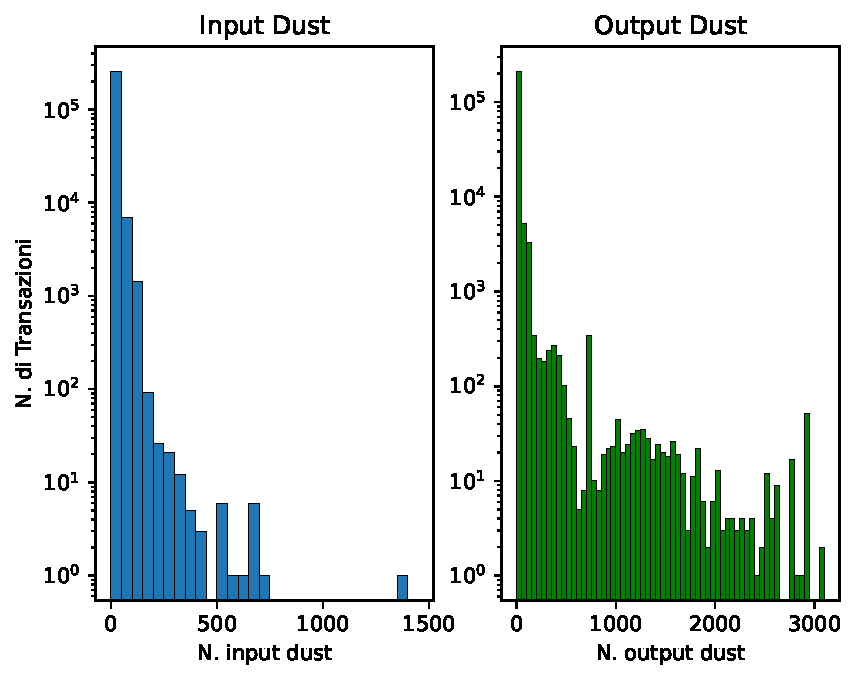
\includegraphics[scale=0.9]{Grafici/distribuzione_dust.pdf}
    \caption{Distribuzione numero input dust(sinistra) e output dust(destra). Intervalli di ampiezza 50, primo intervallo [1, 50]}
    \label{fig:dust_distribuzione}
\end{figure}
\FloatBarrier 
Entrambi gli istogrammi mostrano come siano molto frequenti le transazioni presenti nel primo intervallo di ampiezza [1, 50]. Nel primo grafico notiamo anche che le transazioni con un elevato numero di input dust risultino poco frequenti. Al contrario del primo grafico, il secondo mostra come siano presenti tante transazioni che generano un elevato numero di output dust. Dall'analisi di questi due grafici inoltre possiamo già intuire che diversi output dust generati non vengano successivamente spesi.

In tutte le analisi successive viene considerato solo il dust generato con script diverso da OP\_RETURN. Questa scelta è motivata dal fatto che gli output con questo script non possono essere spesi, questa tipologia di dust quindi non può avere effetti sulla de-anonimizzazione; inoltre chi lo sta generando sicuramente non sta attuando un Dust Attack.

Il grafico \ref{fig:dust_created} mostra la distribuzione nel tempo del dust spendibile.
\begin{figure}[h!]
    \centering
    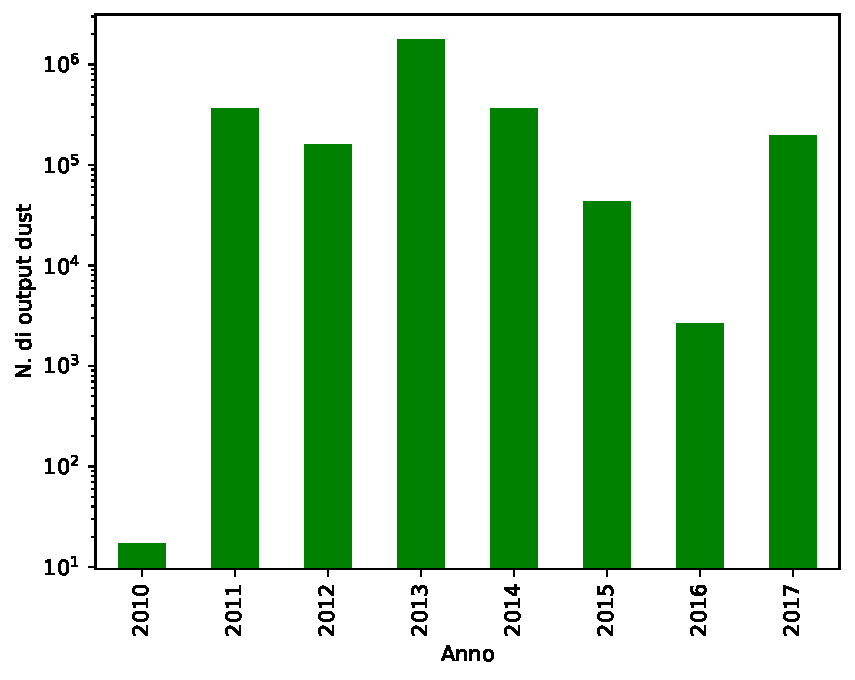
\includegraphics[scale=0.9]{Grafici/dust_created_year.pdf}
    \caption{Creazione dust nel tempo}
    \label{fig:dust_created}
\end{figure}
\FloatBarrier 
Dal grafico è possibile notare che già dal 2010 sono comparsi i primi output dust, anche se in quantità molto ridotta. Possiamo osservare un rapido aumento tra il 2010 e il 2011, solo nel mese di luglio dell'anno 2011 infatti sono stati generati più di 27 000 output dust.

Il picco della generazione di dust è presente nel 2013, dove sono stati trovati pattern interessanti di transazioni legate "a catena"; nel paragrafo successivo verranno approfonditi questi schemi. Dopo il picco del 2013 osserviamo una diminuzione negli anni fino al 2017 dove si assiste ad una ricrescita. Bisogna però specificare che la maggior parte del dust generato nel 2017 proviene da due address: $1Enjoy1C4bYBr3tN4sMKxvvJDqG8NkdR4Z$ e $1SochiWwFFySPjQoi2biVftXn8NRPCSQC$.

Questi due noti address sono comparsi per la prima volta nel 2014, in concomitanza con le olimpiadi di Sochi in Russia, generando transazioni con circa 750 output di 1 satoshi ciascuno. È importante notare come, nonostante il caos causato in vari forum Bitcoin, la tempesta di spam del 2014 "Enjoy Sochi" abbia lasciato una piccola impronta sulla blockchain; solo 65 transazioni(48 750 output dust) sono state confermate in quell'anno.

L'aspetto singolare di questo fenomeno è che abbiamo visto echi di esso tornare negli anni successivi. Nel 2015 infatti sono state confermate 23 transazioni(1 725 output dust) mentre nel 2017 sono presenti 255 transazioni(191 250 output dust) generate da questi vanity address. Sebbene sia possibile che siano state eseguite dalla stessa entità, che spendeva importi da quegli address anche nel 2018, è anche possibile che queste transazioni fossero state generate nel 2014 e confermate solo nel 2015 e nel 2017. In questi tre anni il fenomeno "Enjoy Sochi" ha generato 343 transazioni per un totale di output dust intorno ai 255 000.

In generale sono stati generati 2 893 877 output dust con script diverso da OP\_RETURN; circa il 48.5\% è stato speso. Quindi la quantità di dust non speso(51.5\%) è paragonabile a quello speso. 

La tabella \ref{tab:dust_spent_unspent} mostra le percentuali negli anni del dust speso e non-speso; il 2009 non è stato considerato perchè non è stato generato alcun output dust in quell'anno. La superiorità del dust non-speso rispetto al dust speso è presente soprattutto negli anni 2011 e 2017, anche se parte del dust del 2017 potrebbe essere stato speso successivamente al 10 Agosto 2017, data dell'ultima transazione del dataset. Il 2010, nonostante il dust non-speso sia l'83\%, non è molto rilevante poichè sono stati generati solo 14 output dust in totale. 
\begin{table}[H]
    \centering
    \begin{tabular}{|c|c|c|c|c|c|c|c|c|}
        \hline
           categoria/anno   & 2010 & 2011 & 2012 & 2013 & 2014 & 2015 & 2016 & 2017\\
        \hline 
         speso &  17\% & 0,2\% & 54\% & 44\% & 76\% & 94,6\% & 95,6\% & 10\% \\
         \hline
         non-speso & 83\% & 99,8\% & 46\% & 56\% & 24\% & 5,4\% & 4,4\% & 90\%  \\
         \hline
    \end{tabular}
    \caption{Dust Speso e Non-Speso negli anni}
    \label{tab:dust_spent_unspent}
\end{table}
\section{Classificazione del dust}
Come descritto nella sezione \ref{algoritmii} gli output dust sono stati suddivisi in quattro categorie:
\begin{enumerate}
    \item \textbf{Successo}: dust speso in transazioni che presentano almeno due address diversi di input, in queste transazioni la fee è diversa dall'importo totale di input;
    \item \textbf{Fallimento}: dust speso in transazioni con un solo address di input, anche se ripetuto più volte;
    \item \textbf{Speciale}: dust speso in possibili transazioni di ``dust collecting", transazioni la cui fee è uguale all'importo totale di input;
    \item \textbf{Non speso}.
\end{enumerate}

I termini "Successo" e "Fallimento" si riferiscono alla possibilità di collegare gli address di input una volta che il dust è stato speso. Nonostante il ``dust-collecting" rappresenti un caso di de-anonimizzazione fallita, poichè gli address di input potrebbero appartenere ad utenti diversi, questa situazione viene separata dalla categoria ``Fallimento" per mostrare se e quanto sia stato utilizzato questo servizio.

Il grafico \ref{fig:dust_year} mostra la distribuzione delle categorie nel corso degli anni.
\begin{figure}[h!]
    \centering
    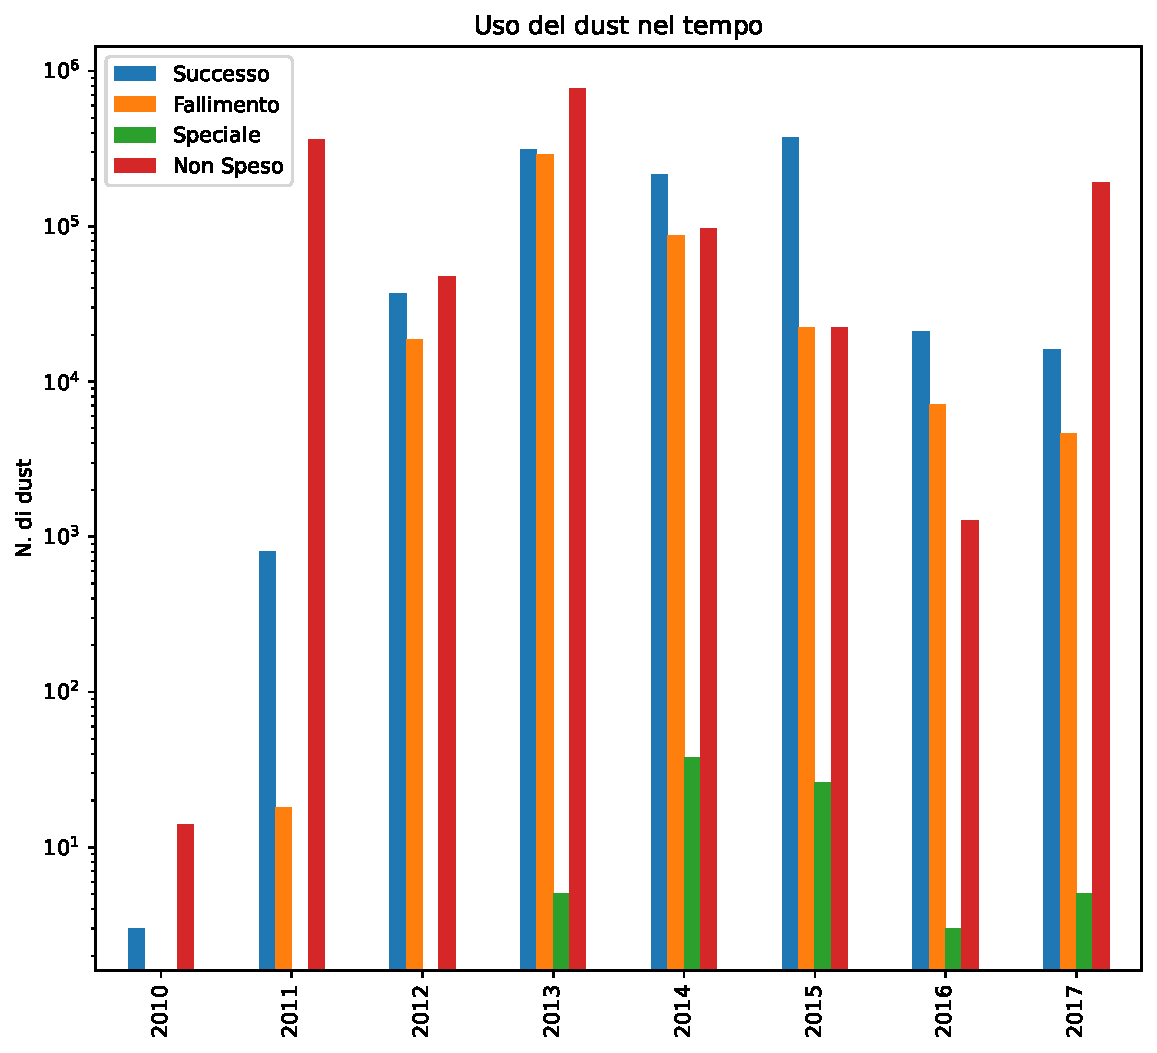
\includegraphics[scale=0.6]{Grafici/uso_del_dust_new.pdf}
    \caption{Uso del dust nel tempo}
    \label{fig:dust_year}
\end{figure}
\FloatBarrier

Non solo possiamo constatare graficamente quanto detto prima sulla differenza tra dust speso e non speso, ma possiamo anche fare due importanti riflessioni. 

La prima riflessione riguarda l'uso del servizio di ``dust collecting", risulta evidente quanto poco esso sia stato utilizzato. È importante notare che il dust della categoria ``Speciale" non necessariamente è legato a Dust-B-Gone, questa categoria infatti è presente anche nel 2017 nonostante il servizio sia stato ufficialmente chiuso nel 2016. Infatti rientrano in questa categoria anche gli utenti che decidono di propria iniziativa di spendere tutto il dust in fee. In generale infatti non è possibile distinguere una transazione di ``dust-collecting" da una transazione generata da un singolo utente, tuttavia il numero di dust della categoria ``Speciale" permette di capire quanto sia stato utilizzato questo servizio, infatti il numero di dust spesi in transazioni di ``dust-collecting" può essere al massimo uguale al numero totale di dust della categoria ``Speciale".  

La seconda riflessione invece riguarda la tendenza a spendere il dust con almeno un altro address, in particolare notiamo un netto distacco nel 2015 dove la categoria ”Successo” è dell’ordine di $10^4$ mentre ”Fallimento” dell’ordine di $10^3$. In generale questa informazione è molto importante perchè dimostra come il dust possa essere efficace per la de-anonimizzazione di un wallet, ovvero capire che più address appartengano ad un medesimo utente.

Una volta constatata la presenza di transazioni con input dust e con almeno due address diversi, la fase seguente è l'analisi delle transazioni. 
\section{Classificazione delle Transazioni}
Considereremo tre categorie di transazioni: 
\begin{itemize}
    \item \textbf{2+ address}: transazioni che presentano almeno due address di input differenti, la fee però è diversa dall'importo totale di input;
    \item \textbf{1 address}: transazioni con un singolo address di input;
    \item \textbf{speciale}: transazioni dove l'importo totale di input è uguale alla fee.
\end{itemize}

In totale il dust è stato speso in 263 963 transazioni, la tabella \ref{tab:tx_categories} mostra la percentuale delle transazioni nelle tre categorie, la tabella \ref{tab:tx_categories_year} mostra la distribuzione negli anni.
\begin{table}[H]
    \centering
    \begin{tabular}{|c|c|}
        \hline
        2+ address & 63,2\%\\
        \hline
        1 address & 36,7\%\\
        \hline
        speciale & 0.1\%\\
        \hline
    \end{tabular}
    \caption{Transazioni delle tre categorie}
    \label{tab:tx_categories}
\end{table}
\begin{table}[H]
    \centering
    \begin{tabular}{|l|c|c|c|c|c|c|c|c|}
        \hline
            categoria/anno  & 2010 & 2011 & 2012 & 2013 & 2014 & 2015 & 2016 & 2017\\
        \hline 
         2+ address(\%) & 100 & 93 & 55,6 & 68,4 & 55,9 & 64,5 & 62,7 & 75 \\
         \hline
         1 address(\%) & 0 & 7 & 44,4 & 31,5 & 44,09 & 35,4 & 37,2 & 24,7  \\
         \hline
         speciali(\%) & 0 & 0 & 0 & 0,1 & 0,01 & 0,1 & 0,1 & 0,3 \\
         \hline
    \end{tabular}
    \caption{Transazioni delle tre categorie nel tempo}
    \label{tab:tx_categories_year}
\end{table}
Dalle tabelle \ref{tab:tx_categories} \ref{tab:tx_categories_year} confermiamo quanto detto prima, la prevalenza a spendere il dust in transazioni con almeno due address diversi e lo scarso utilizzo di servizi come Dust-B-Gone. Siccome sono presenti solo 17 transazioni della terza categoria 
\subsection{Categoria 1 Address}
La categoria "1 address" è stata ulteriormente suddivisa in due classi:
\begin{itemize}
    \item \textbf{NOD}(Not Only Dust): transazioni che presentanto almeno un input con importo $>$ 545  
    \item \textbf{OD}(Only Dust): transazioni con soli input dust.
\end{itemize}

Dalla tabella \ref{tab:OD_NOD_failed} possiamo dedurre che il fallimento nella de-anonimizzazione sia dovuto principalmente a quegli address che presentano un saldo positivo, ovvero un bilancio complessivo $>$ 0. In questo caso gli address hanno potuto spendere il dust con altri input provenienti tutti dal medesimo address, impedendo ad un possibile attaccante di creare un cluster da associare ad un unico utente.
\begin{table}[H]
    \centering
    \begin{tabular}{|c|c|c|}
        \hline
            NOD  & 92 712 & 95,5\%\\
        \hline 
            OD  & 4328 & 4,5 \%\\
        \hline
    \end{tabular}
    \caption{Classificazione OD e NOD}
    \label{tab:OD_NOD_failed}
\end{table}
Interessante invece è il secondo gruppo, in particolare due address appartenenti ad esso:
\begin{itemize}
    \item \textit{1JwSSubhmg6iPtRjtyqhUYYH7bZg3Lfy1T}
    \item \textit{1PEDJAibfNetJzM289oXsW1qLAgjYDjLgN}
\end{itemize}

Il fatto interessante del primo address è che che la sua chiave privata è stata compromessa \footnote{fonte:\url{https://privatekeys.pw/address/bitcoin/1JwSSubhmg6iPtRjtyqhUYYH7bZg3Lfy1T}}, questo consente a chiunque di riscattare bitcoin non appena vengono inviati a questo address. Questo address è tipicamente destinatario di transazioni di 2936 output dust, tutti gli importi sono destinati ad esso. Questo address fornisce quindi un metodo di scrivere dati arbitrari sulla blockchain minimizzando i costi.

Caso anomalo invece riguarda il secondo address, rinominato \textit{1PED} per semplicità. Questo address, come riportato in \cite{dustAnalisi} è un noto gambler di Satoshi Dice, la singolarità però deriva da alcune transazioni che ha generato. In queste transazioni infatti è presente un solo input di 1 satoshi e un solo output, ovviamente sempre di 1 satoshi. Questi singoli satoshi però non provengono da Satoshi Dice ma da altri address che seguono un pattern ben preciso, schematizzato nella figura \ref{fig:1PED}
\begin{figure}[h!]
    \centering
    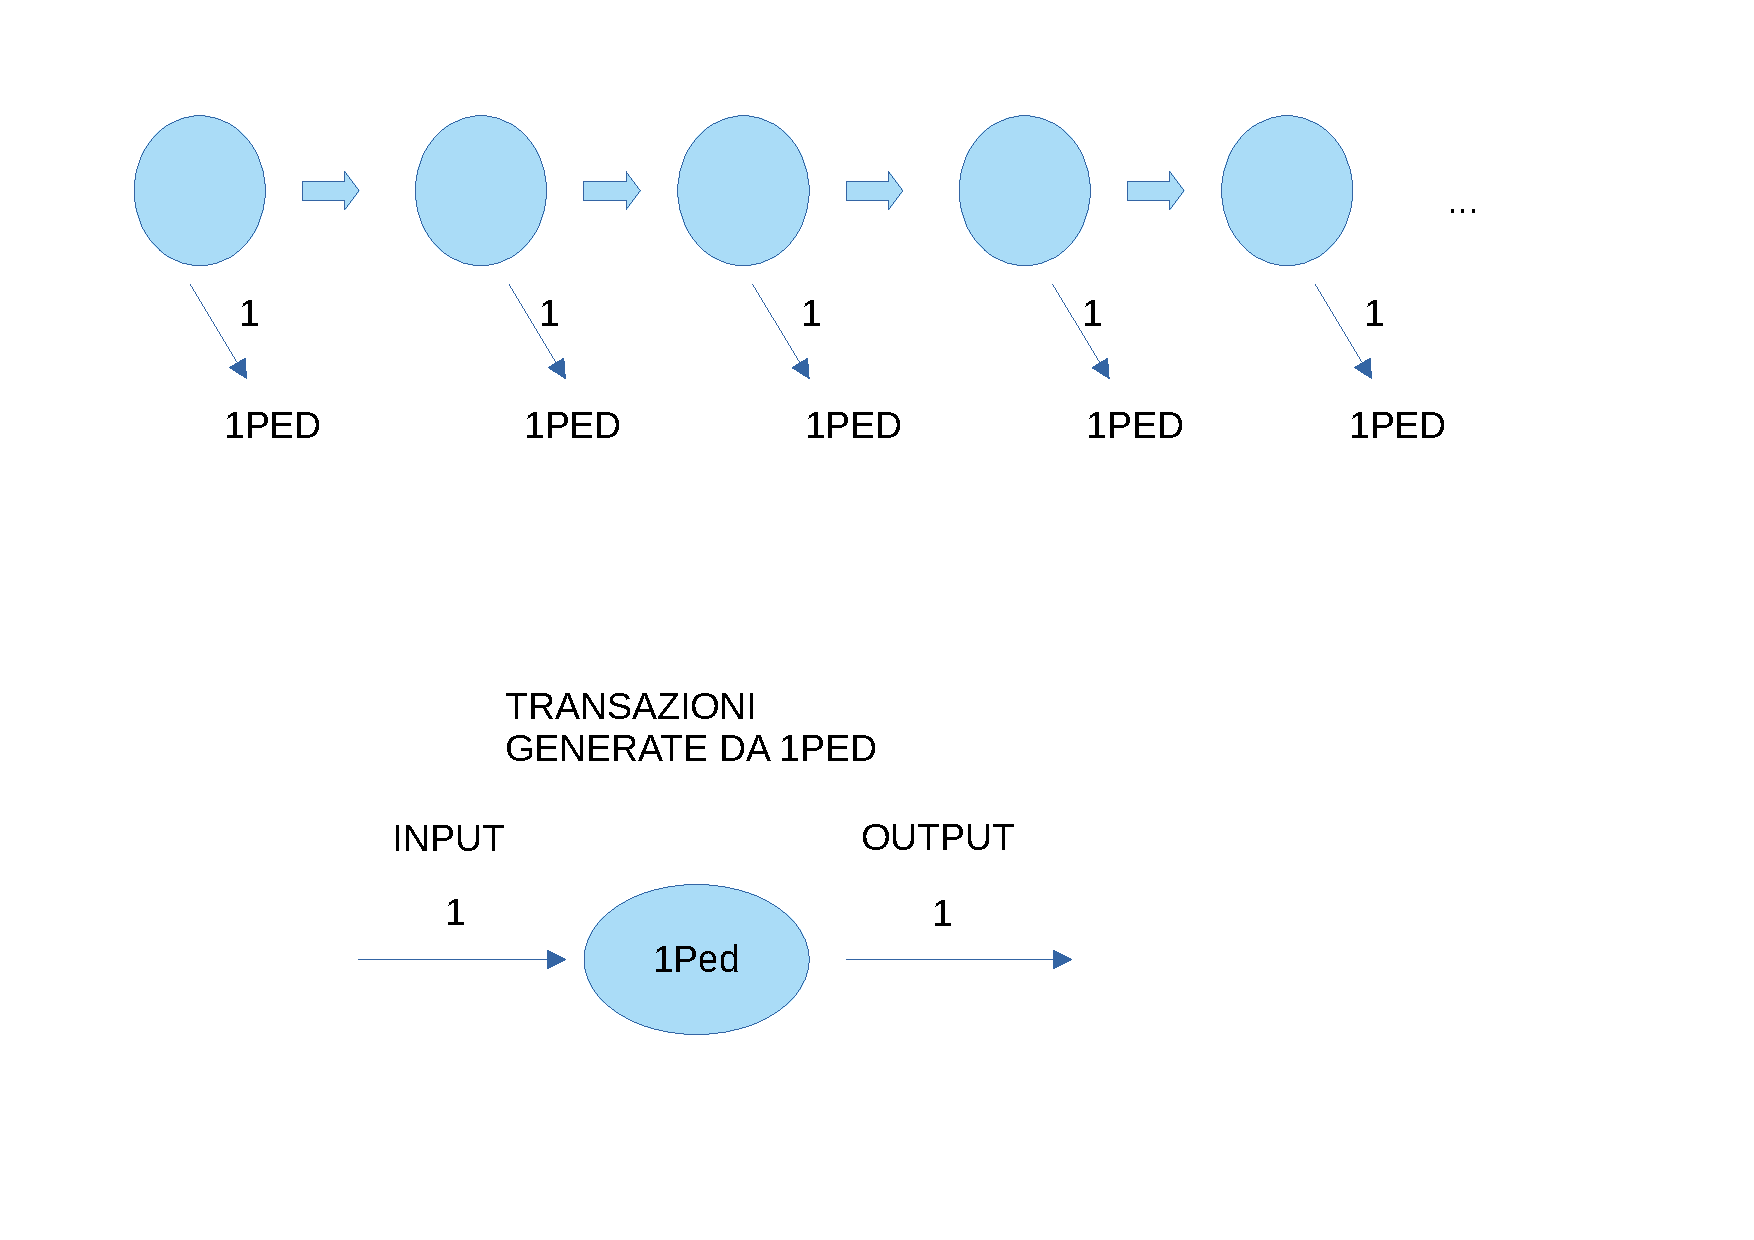
\includegraphics[scale=0.4]{Images/1Ped.pdf}
    \caption{Schema transazioni legate a \textit{1PED}}
    \label{fig:1PED}
\end{figure}
\FloatBarrier
Ogni address, appartenente al pattern, invia due output, 1 satoshi con destinatario \textit{1PED} e un secondo importo che viene inviato ad un altro address che seguirà il medesimo schema; in tutte queste transazioni la fee è sempre di 50 000 satoshi. \textit{1PED} ha generato poi 1835 transazioni con 1 solo satoshi di input e 1 solo satoshi di output, la data è il 10 Marzo 2013 alle ore 16:20. È interessante sottolineare come \textit{1PED} sia riuscito a spendere un singolo satoshi senza la necessità di aggregare il dust con altri input. Questo significa che, nonostante queste transazioni fossero non-standard, il mineri ha comunque deciso di validarle, però sebbene questo comportamento sia anomalo risulta alquanto improbabile che si tratti di Dust Attack. Questa considerazione deriva dal fatto che tutti gli address di output delle transazioni generate da \textit{1PED} sono address nuovi.
\subsection{Categoria 2+ Address}
Una volta esaminate le transazioni ``1 address" il prossimo passaggio è l'analisi delle transazioni della categoria "2+ address". Anche in questo caso vengono mostrati i gruppi OD e NOD. La tabella \ref{tab:OD_NOD_success} mostra come quasi sempre gli importi dust vengano aggregati ad altri importi non-dust.
\begin{table}[H]
    \centering
    \begin{tabular}{|c|c|c|}
        \hline
            NOD  & 166 778 & 99,9\%\\
        \hline 
            OD  & 128 & 0,1 \%\\
        \hline
    \end{tabular}
    \caption{Classificazione OD e NOD}
    \label{tab:OD_NOD_success}
\end{table}
È importante però capire quanto successo abbia avuto la deanonimizzazione causata dal dust, anallizzando soprattutto gli address di input. In particolare è importante capire quanti address diversi ci siano all'interno di una singola transazione, in modo da capire il livello di de-anonimizzazione che il dust permette. Generalmente più address riesco ad unire in un singolo cluster maggiore è il livello di de-anonimizzazione ottenuta, infatti più address associo ad un singolo utente maggiore è la tracciabilità dell'attività di quell'utente.

Il grafico \ref{fig:diff_addr} mostra la distribuzione del numero di address diversi, un notevole numero di transazioni tende ad avere un numero di address nel primo intervallo, ovvero nell'intervallo [2, 50]. È possibile notare come sia presente un elevato numero di transazioni con centinaia address di input, in queste transazioni quindi è stato possibile collegare centinaia di address diversi appartenenti ad un unico utente. Ad esempio la transazione con il maggior numero di address differenti contiene ben 1750 address diversi, in questo caso è stato possibile collegare più di mille address ad un unico utente. In generale la media è di 13 address diversi in una singola transazione. 

 \begin{figure}[h!]
     \centering
     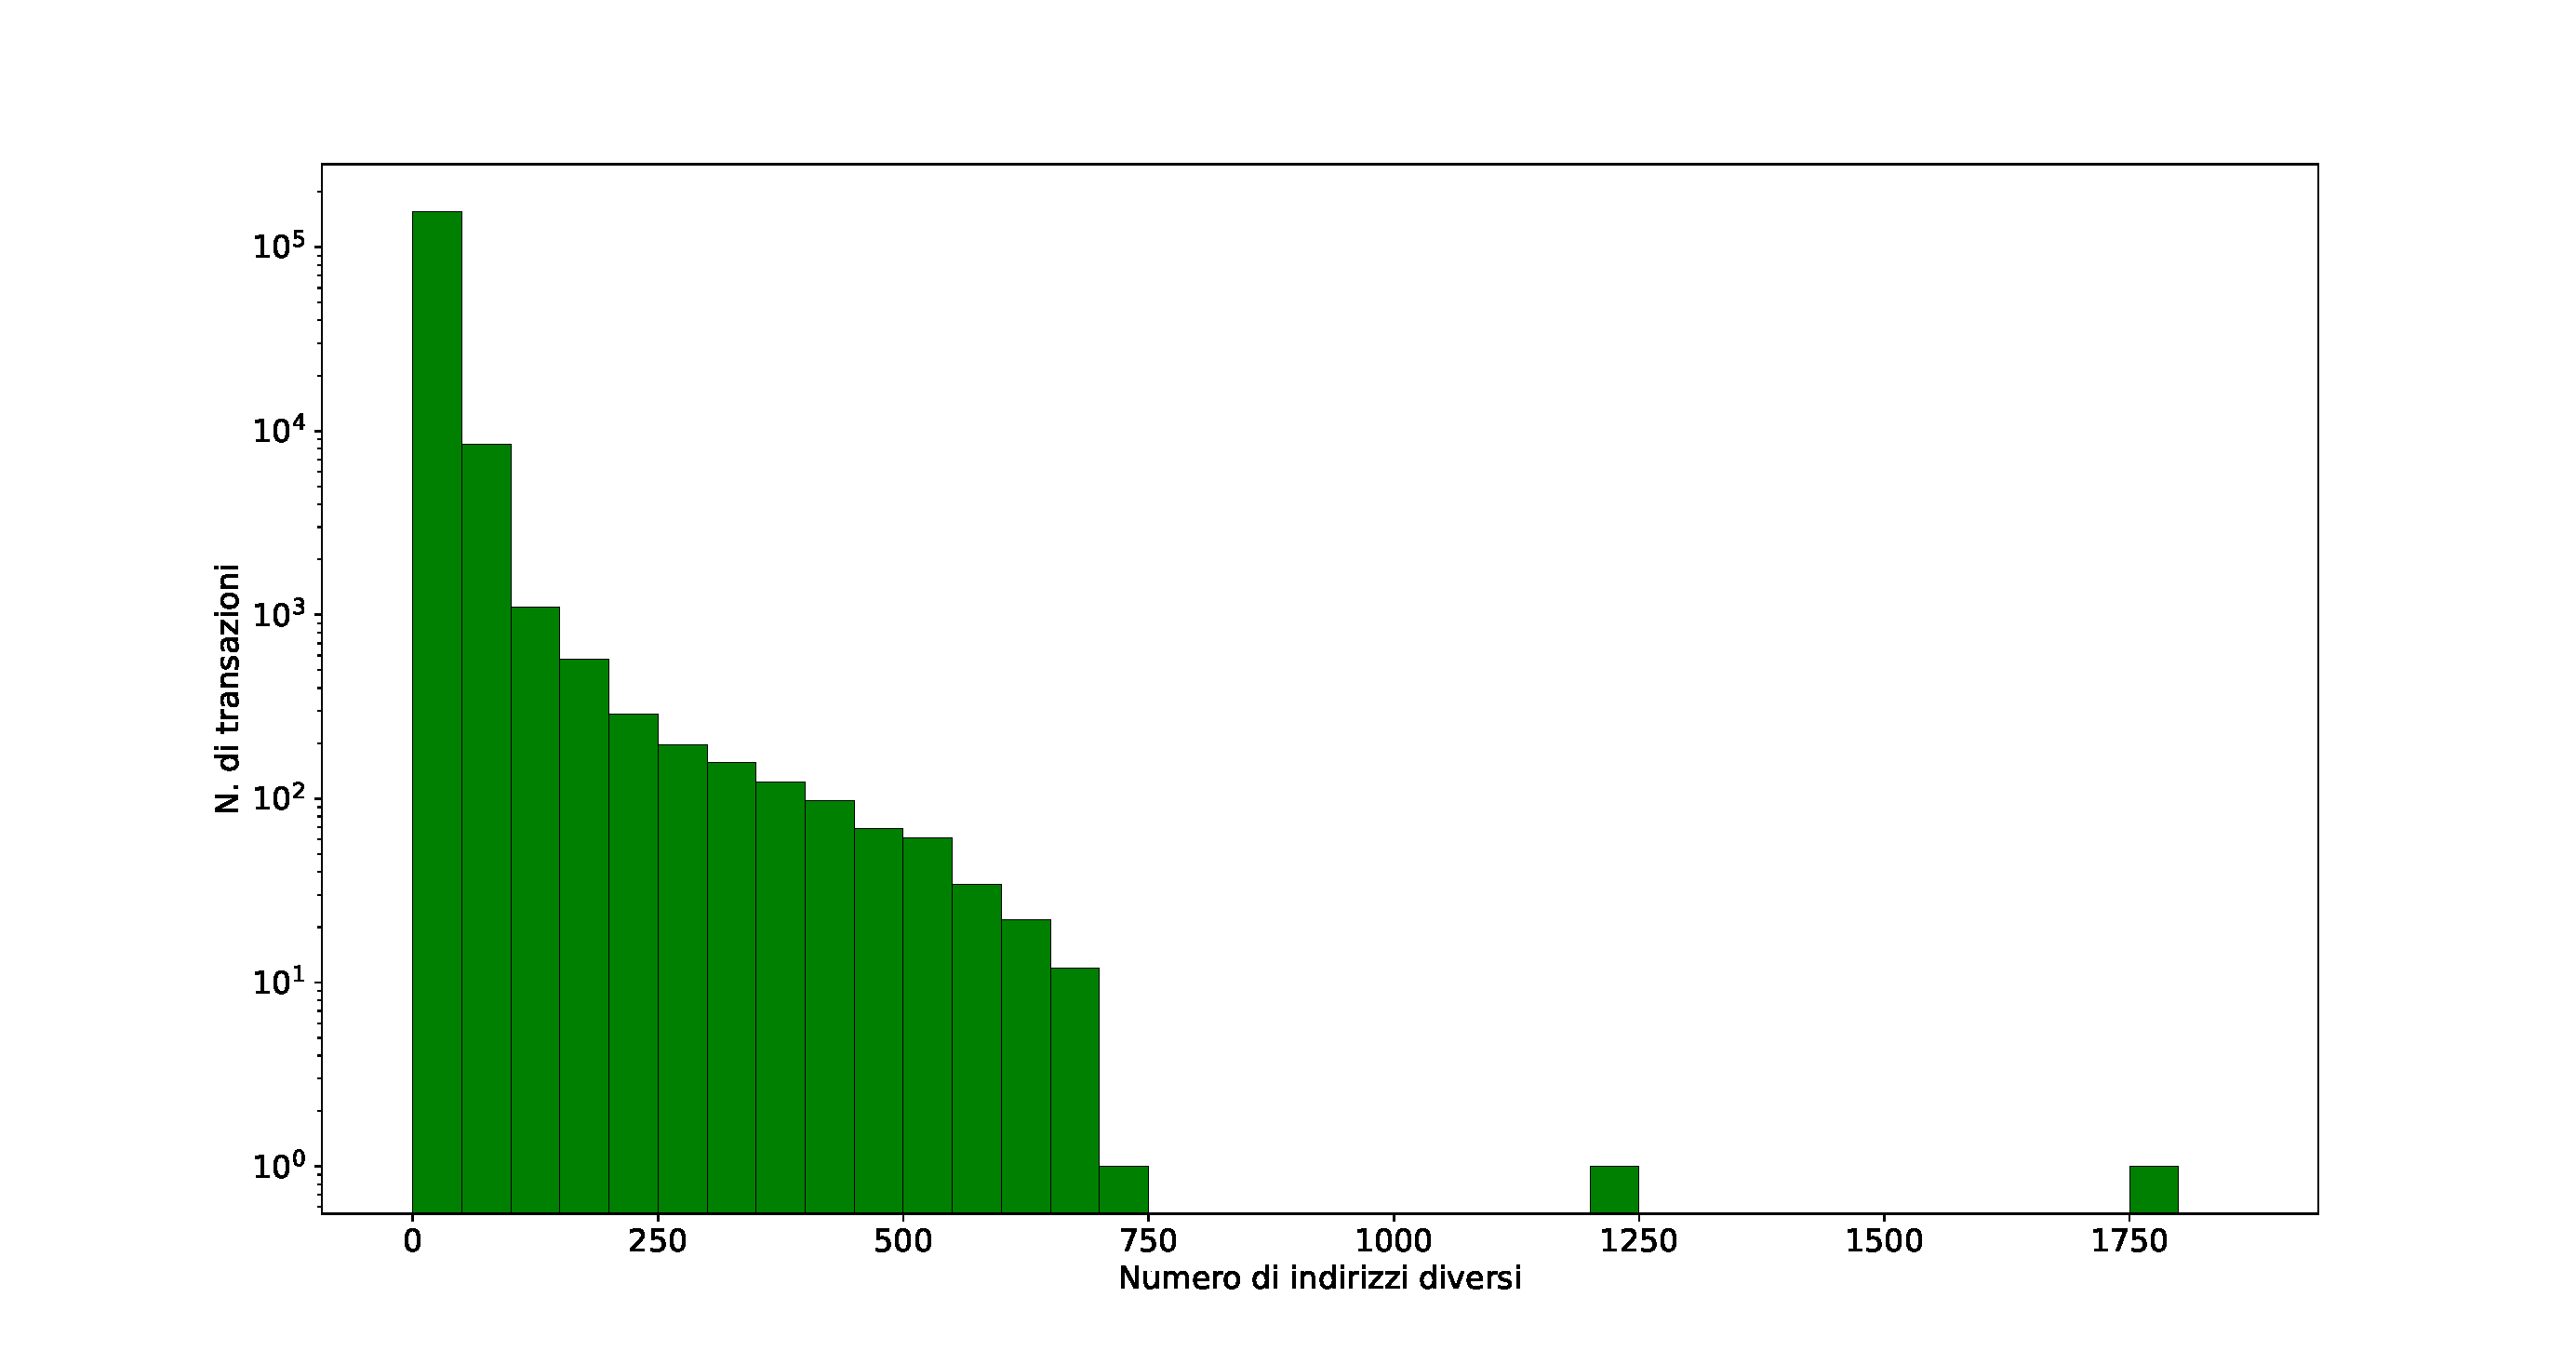
\includegraphics[scale=0.3]{Grafici/num_addr.pdf}
     \caption{Distribuzione numero address differenti. Colonne di ampiezza 50, la prima colonna rappresenta l'intervallo (1, 50]}
     \label{fig:diff_addr}
 \end{figure}
\FloatBarrier
Questi dati sembrerebbero confermare l'utilità del Dust Attack, tuttavia è importante precisare che stessi address possano apparire in più transazioni, quindi diverse transazioni potrebbero riferire i medesimi address di input, portando ad una de-anonimizzazione ripetuta. 

Nonostante siano stati generati 2 893 877 output dust gli address a cui sono stati inviati sono 1 059 836 e solo il 29\%(312 114) lo ha speso. Di questo 29\% abbiamo che 259 252 hanno speso il dust in transazioni della categoria "2+ address" anche se 4 270 address hanno generato anche transazioni nella categoria "1 address". Una particolarità interessante delle transazioni che hanno generato il dust "Successo" è che in molti casi erano presenti tra gli output dust address nuovi, ovvero address che non erano mai comparsi sulla blockchain. 

Ci sono 98 198 transazioni che generano almeno un dust della categoria "Successo", circa il 59\%(58 146) non presenta address nuovi tra gli output. Come spiegato nella sezione \ref{dstatt} è molto improbabile che un attaccante invii del dust ad un address nuovo, proprio perchè risulterebbe strano de-anonimizzare un address mai visto. Nella fase finale della procedura di analisi quindi sono state considerate queste transazioni così da trovare dei pattern interessanti di possibili Dust Attack di successo; nel paragrafo successivo verranno approfonditi due possibili schemi di Dust Attack.  
\section{Analisi di Pattern Interessanti}
In generale è complicato affermare con certezza se un address stia compiendo un Dust Attack, però abbiamo individuato due schemi, con certe proprietà, che rappresentano probabilmente un Dust Attack e sono caratterizzati da alcune proprietà. La proprietà più importante riguarda l'assenza di address nuovi tra gli output dust, proprio perchè è alquanto improbabile tentare di de-anonimizzare un address mai visto fino a quel punto.

Il primo pattern, sintetizzato in \ref{fig:schema1}, risulta molto simile al caso 1PED. Esistono diversi address legati a catena che generano transazioni bi-output. Il secondo output, inviato sempre al solito address probabilmente l'address di un attaccante, viene speso dall'attaccante per generare transazioni contenenti solo output dust. Inoltre l'attaccante, nell'immagine l'ovale rosso, non compare mai nella catena dei finanziatori, rappresentata dai cerchi azzurri.
\begin{figure}[h!]
    \centering
    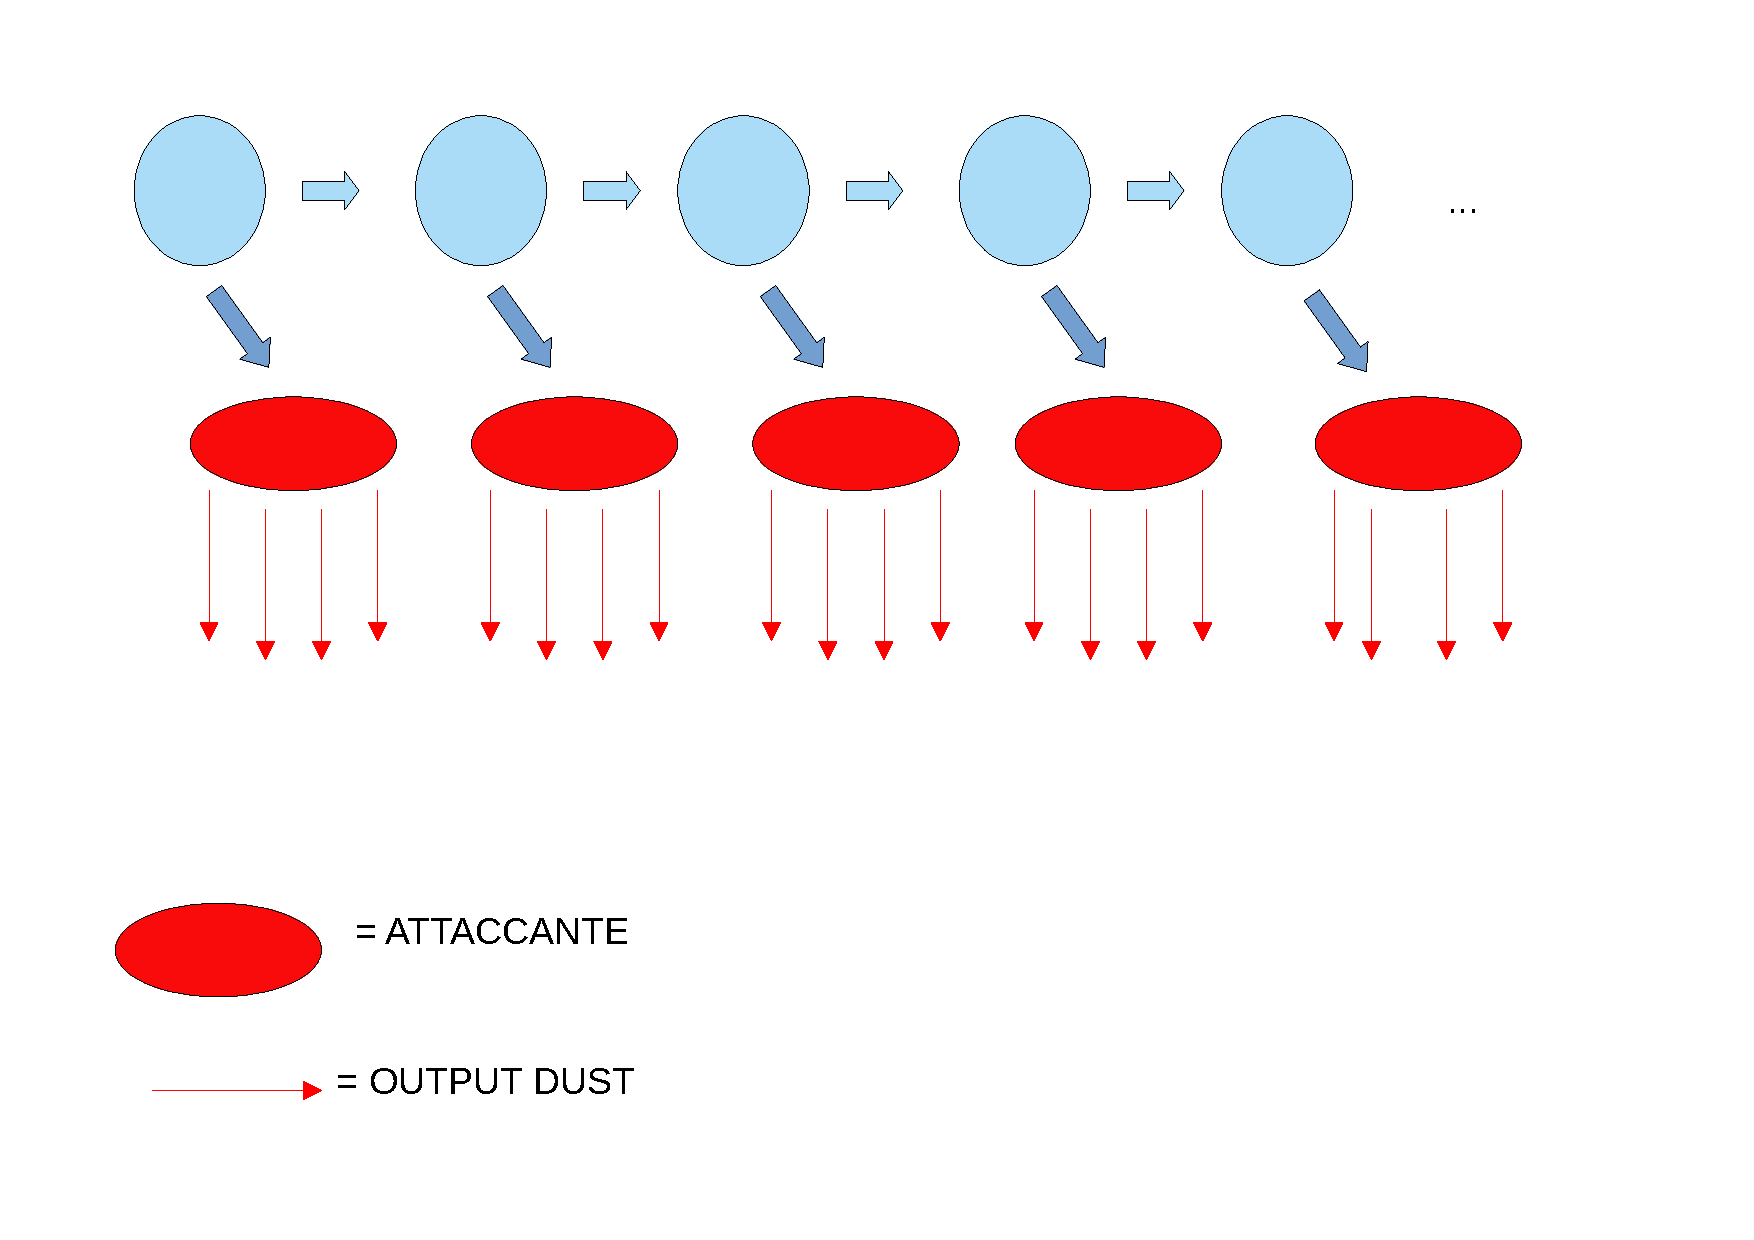
\includegraphics[scale=0.4]{Images/dust_attack1.pdf}
    \caption{Pattern ``Un finaziatore un attaccante"}
    \label{fig:schema1}
\end{figure}
\FloatBarrier
Altre proprietà importanti di questo pattern sono: fare riferimento ad un unico finanziatore, generare sempre lo stesso numero di output dust, avere sempre il medesimo importo di input e infine tutte esegue le transazioni sono eseguite in un breve intervallo di tempo. Questo schema è stato scoperto tramite l'address \textit{1DiRy9Giiq1GCkAD7VMSrXoKVe2dimnovm}, finanziato da \textit{1Nj3AsYfhHC4zVv1HHH4FzsYWeZSeVC8vj}. Inoltre sono presenti altri address che seguono lo stesso schema, pagati sempre dallo stesso finanziatore di $1DiRy$. Questo significa che il pattern appena enunciato può essere eseguito in parallelo utilizzano diversi address attaccanti. Potrebbero esserci in aggiunta più finanziatori che inviano denaro a più attaccanti. Per esempio questo address \textit{16JLbXYe5xmxGNX8hiqooyTUJnhitNNqTh} ha ricevuto fondi da \textit{1NPfnbqZAMUnGuNuYwVZdCN4qVzUq4ejG4}, l'aspetto interessante però è che il numero di output dust, l'importo dust inviato, l'importo input speso sono esattamente uguali a quelli usati da \textit{1Diry}; questo fatto fa ipotizzare che probabilmente questi address appartengano allo stesso utente. Ovviamente possono esserci eccezioni a questi due esempi trovati, per esempio avere più finanziatori o più attaccanti in una stessa catena, inoltre gli importi e il numero di output dust potrebbero avere una natura più casuale. In generale si potrebbero ipotizzare diverse variazioni di questo pattern, anche se non ne abbiamo verificato la presenza.

Il secondo pattern riguarda le transazioni "a catena" del 2013 citate nel paragrafo precedente; questo schema è stato scoperto tramite l'address \textit{1JYvvL67LrSGCG77cy4rmpUXCFfSub4JkG} (rinominato \textit{1JYvv}), Ogni address della catena invia centinaia o migliaia di output dust e il resto dell'importo viene inviato al prossimo address che seguirà lo stesso schema. La singolarità di questo modello è che gli address della catena, ad eccezione del primo, vengono utilizzati solo per eseguire quell'unica transazione; non verranno mai più riutilizzati.
\begin{figure}[h!]
    \centering
    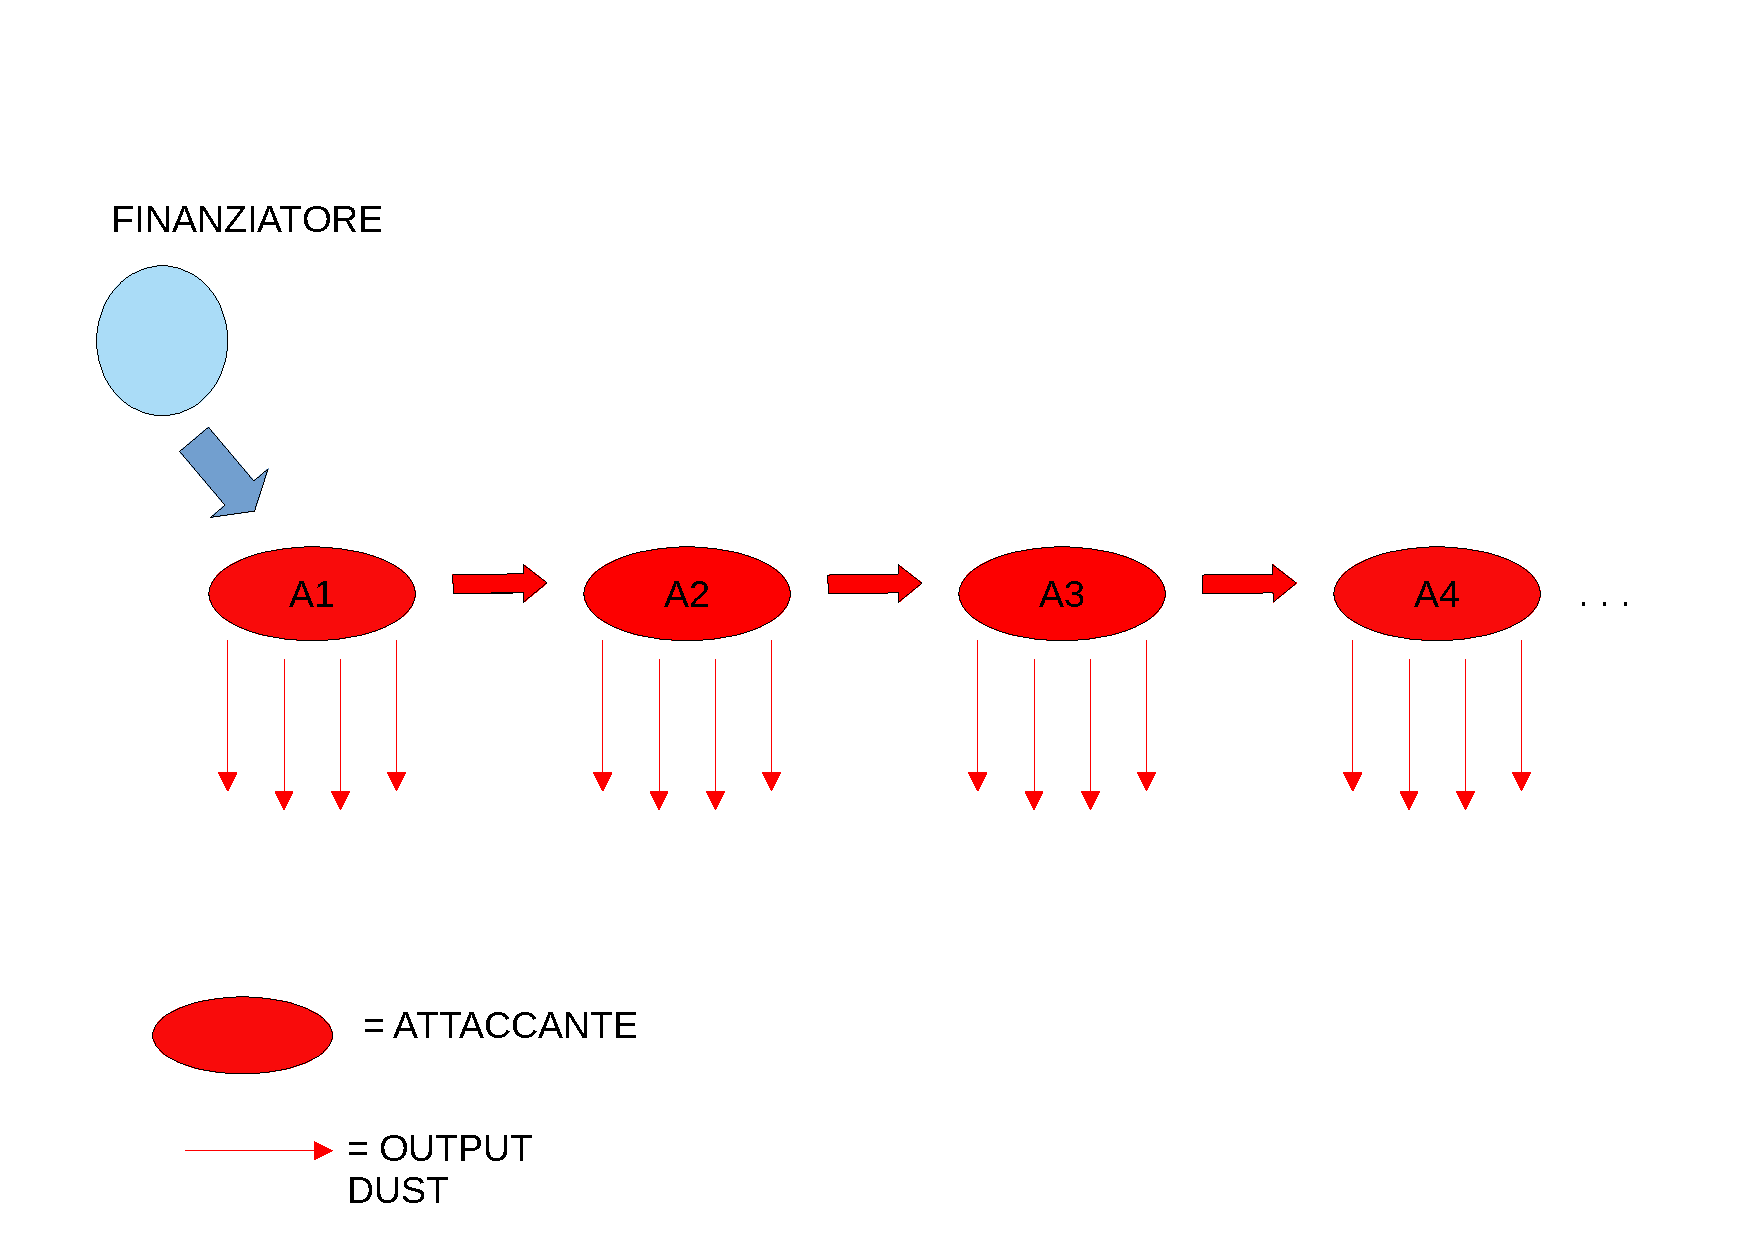
\includegraphics[scale=0.4]{Images/dust_attack2.pdf}
    \caption{Pattern ``Un finanziatore più attaccanti"}
    \label{fig:schema2}
\end{figure}
\FloatBarrier
Consideriamo ad esempio l'address A3 della figura \ref{fig:schema2}. A3 riceve un importo da A2 e utilizza parte di questo importo per inviare centinaia o migliaia di output dust, il resto dell'importo, esclusa la fee, viene inviato ad A4 che seguirà il medesimo schema. Questo discorso però non si applica all'address che inizia questo pattern(A1), per esempio l'address 1JYvv ha cominciato una serie di catene con questo modello.

Potrebbe essere interessante in futuro capire quanti address abbiano seguito schemi di questi tipo e se ci siano altri fini oltre a quello di un possibile Dust Attack.
\chapter{Conclusioni e sviluppi futuri}
In questa tesi abbiamo definito il Dust Attack, mostrando gli obiettivi dell'attacco, le conseguenze e le possibili contromisure. É stato analizzato il dust, escludendo gli importi dust generati da Satoshi Dice, in particolare é stato mostrato come il dust abbia permesso la creazione di diversi cluster di address in varie transazioni, dimostrando come il Dust Attack possa risultare efficace nella de-anonimizzazione dei wallet in Bitcoin. Infine sono stati descritti due pattern che hanno generato un elevato numero di output dust inviato ad address non-nuovi e che potrebbero rappresentare degli schemi di Dust Attack. 

Alcuni sviluppi futuri di questo lavoro che possono essere suggeriti riguardano proprio questi due pattern introdotti nel paragrafo \ref{pattern}. Potrebbero essere svolte ulteriori analisi per identificare quanti pattern di questo tipo siano presenti negli anni e se vengano utilizzati solo per eseguire un Dust Attack. Potrebbe essere interessante anche capire se gli address a cui viene inviato il dust siano scelti in modo casuale o se siano scelti address con determinate caratteristiche. 

Un'altra idea potrebbe essere il confronto tra il Dust Attack ed altri attacchi di de-anonimizzazione che non si basano sull'invio di dust. In particolare potrebbe essere interessante analizzare i cluster ottenuti mediante importi dust e i cluster ottenuti con altre tipologie di analisi della blockchain, così da capire se il Dust Attack abbia permesso l'individuazione di cluster non osservabili utilizzando gli attacchi classici.

% Mostra bibliografia
\printbibliography[heading=bibintoc]

%``"
\end{document}
